\documentclass{article}

% ============================================================
% Packages
% ============================================================

\usepackage[margin=1in]{geometry}
\usepackage{graphicx}
\usepackage{booktabs}
\usepackage{multirow}
\usepackage{tabularx}
\usepackage{array}
\usepackage{threeparttable}
\usepackage{longtable}

% Packages for Tables 3--7 and Figures 1--2 (Results 3.2--3.6)
% (booktabs/multirow are already loaded above; loading them again is harmless)
\usepackage{booktabs,multirow,pifont,adjustbox}
\usepackage{pgfplots}
\usepgfplotslibrary{groupplots}
\usetikzlibrary{calc}
\usetikzlibrary{arrows.meta,positioning}   % Figure 1 (flowchart)
\pgfplotsset{compat=1.18}
% low risk = green, high risk = red
\definecolor{kmlow}{HTML}{3A9D5D}
\definecolor{kmhigh}{HTML}{E2574C}
% KM text is set in Times (ptm) regardless of the body font: Computer Modern 7 pt (cmr7) is wide
% enough that the at-risk numbers run into each other. Keeps main.tex and the standalone PDF identical.
\providecommand{\kmsmall}{\fontfamily{ptm}\fontsize{7}{8.4}\selectfont}
\providecommand{\kmlabel}{\fontfamily{ptm}\fontsize{8}{9.6}\selectfont}
\providecommand{\kmletter}{\fontfamily{ptm}\fontsize{10}{12}\selectfont\bfseries}
\tikzset{
  kmlowline/.style={color=kmlow, line width=1pt},
  kmhighline/.style={color=kmhigh, line width=1pt}}
\pgfplotsset{
  kmaxis/.style={
    scale only axis, width=56.3mm, height=40mm, xmin=0, ymin=0, ymax=1.02,
    ytick={0,0.2,0.4,0.6,0.8,1}, yticklabel style={/pgf/number format/.cd, fixed, fixed zerofill, precision=1},
    xticklabel style={/pgf/number format/1000 sep={}},
    xlabel={Time (days)}, ylabel={Survival probability}, axis lines=left, axis line style={-},
    tick align=outside, clip=false, tick label style={font=\kmsmall}, label style={font=\kmlabel},
    title style={font=\kmlabel, align=center, yshift=0.5mm}}}

% X column: left-aligned
\newcolumntype{Y}{>{\raggedright\arraybackslash}X}

% ============================================================
% Document information
% ============================================================

\title{SCLC Multimodal Survival Prediction}
\author{YoungChae Ha \and YeonJin Park}
\date{September 2026}

% ============================================================
% Document
% ============================================================

\begin{document}

\maketitle

\section{Introduction}


% ============================================================
% Figure 1
% Study population and nested cross-validation (fig1_patient_flowchart_nested_simple.tex)
% ============================================================

\begin{figure}[htbp]
\centering
\begin{adjustbox}{max width=\textwidth}
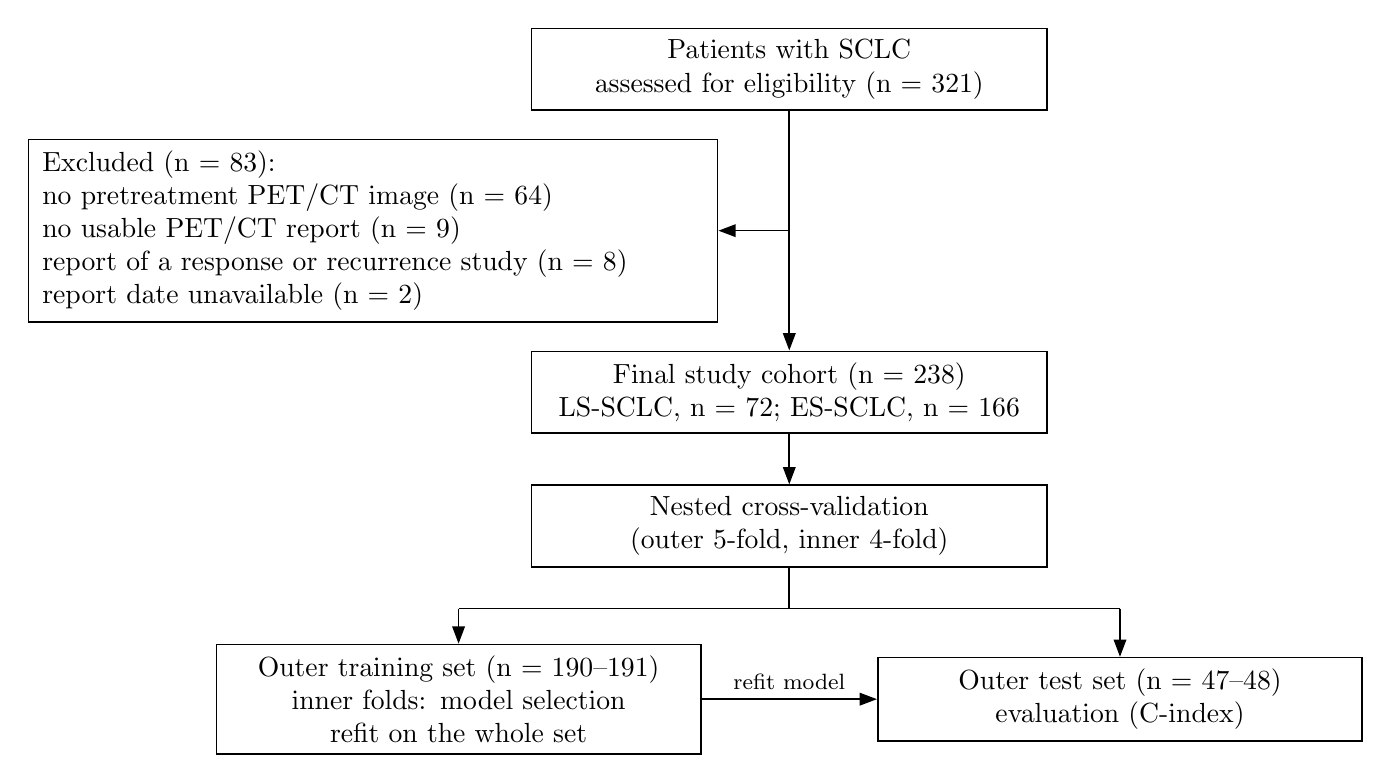
\begin{tikzpicture}[x=1cm,y=1cm,
  box/.style={draw=black, line width=0.6pt, fill=white, align=center,
              inner xsep=5pt, inner ysep=4pt, text width=#1},
  box/.default=62mm,
  excl/.style={box=84mm, align=left},
  arr/.style={draw=black, line width=0.6pt, -{Triangle[length=2.2mm,width=1.6mm]}},
  line/.style={draw=black, line width=0.6pt},
]

% ---------------- 선정 ----------------
\node[box] (all) at (0,0)
  {Patients with SCLC\\ assessed for eligibility (n = 321)};

\node[excl, anchor=east] (ex) at (-0.9,-2.05)
  {Excluded (n = 83):\\
   no pretreatment PET/CT image (n = 64)\\
   no usable PET/CT report (n = 9)\\
   report of a response or recurrence study (n = 8)\\
   report date unavailable (n = 2)};

\node[box] (final) at (0,-4.1)
  {Final study cohort (n = 238)\\ LS-SCLC, n = 72; ES-SCLC, n = 166};

% ---------------- nested 교차검증 ----------------
\node[box] (cv) at (0,-5.8)
  {Nested cross-validation\\ (outer 5-fold, inner 4-fold)};

\node[box=58mm] (otr) at (-4.2,-8.0)
  {Outer training set (n = 190--191)\\ inner folds: model selection\\ refit on the whole set};
\node[box=58mm] (ote) at (4.2,-8.0)
  {Outer test set (n = 47--48)\\ evaluation (C-index)};

% ---------------- 화살표 ----------------
\draw[arr] (all) -- (final);
\draw[arr] (0,-2.05) -- (ex.east);
\draw[arr] (final) -- (cv);
\draw[line] (cv.south) -- (0,-6.85);
\draw[line] (-4.2,-6.85) -- (4.2,-6.85);
\draw[arr] (-4.2,-6.85) -- (otr.north);
\draw[arr] (4.2,-6.85) -- (ote.north);
\draw[arr] (otr.east) -- node[above, font=\footnotesize] {refit model} (ote.west);

\end{tikzpicture}
\end{adjustbox}
\caption{Patient selection and nested cross-validation. In each outer fold, model settings were selected by inner 4-fold cross-validation within the training set, and the model refit on the entire training set was applied once to the test set; each patient was tested exactly once. ES = extensive stage, LS = limited stage, SCLC = small cell lung cancer}
\label{fig:flowchart}
\end{figure}


% ============================================================
% Table 1
% Baseline characteristics of the study cohort
% ============================================================

\begingroup
\small
\renewcommand{\arraystretch}{1.05}
\setlength{\tabcolsep}{4pt}
\setlength{\LTleft}{0pt}
\setlength{\LTright}{0pt}
\begin{longtable}{
  >{\raggedright\arraybackslash}p{2.1in}
  >{\centering\arraybackslash}p{1.25in}
  >{\centering\arraybackslash}p{1.25in}
  >{\centering\arraybackslash}p{1.25in}
}
\caption{Baseline characteristics of the study cohort, stratified by disease stage}
\label{tab:baseline} \\
\toprule
Characteristic & Overall (N=238) & Limited stage (N=72) & Extensive stage (N=166) \\
\midrule
\endfirsthead
\multicolumn{4}{l}{\small\textit{Table \thetable\ continued from previous page}} \\
\toprule
Characteristic & Overall (N=238) & Limited stage (N=72) & Extensive stage (N=166) \\
\midrule
\endhead
\midrule
\multicolumn{4}{r}{\small\textit{Continued on next page}} \\
\endfoot
\bottomrule
\endlastfoot
Age at diagnosis, years & 70.5 [64.0--76.0] & 70.0 [63.0--75.2] & 71.0 [64.2--76.0] \\
Smoking, pack-years\textsuperscript{a} & 43.0 [30.0--55.0] & 40.0 [35.0--50.0] & 45.0 [30.0--55.0] \\
Hemoglobin, g/dL & 12.5 [11.6--13.9] & 12.9 [11.9--14.1] & 12.4 [11.5--13.7] \\
White blood cell count, /\textmu L & 7700.0 [6290.0--9560.0] & 7180.0 [6307.5--8610.0] & 8000.0 [6290.0--9900.0] \\
LDH, U/L & 522.0 [413.0--761.5] & 429.0 [358.8--570.5] & 583.0 [437.0--1032.0] \\
FVC, \% predicted & 88.0 [76.5--99.0] & 89.5 [81.0--99.0] & 87.0 [75.0--99.0] \\
FEV1, \% predicted & 83.5 [69.0--97.0] & 89.0 [72.0--97.0] & 81.0 [68.5--97.0] \\
DLCO (adjusted), \% predicted & 88.0 [71.2--103.8] & 89.0 [77.5--104.8] & 87.0 [70.0--101.5] \\
Sex & & & \\*
\quad Male & 208 (87) & 67 (93) & 141 (85) \\*
\quad Female & 30 (13) & 5 (7) & 25 (15) \\
ECOG performance status & & & \\*
\quad 0 & 25 (11) & 9 (12) & 16 (10) \\*
\quad 1 & 184 (77) & 55 (76) & 129 (78) \\*
\quad 2 & 22 (9) & 5 (7) & 17 (10) \\*
\quad 3 & 7 (3) & 3 (4) & 4 (2) \\
mMRC dyspnea scale & & & \\*
\quad 0 & 14 (6) & 4 (6) & 10 (6) \\*
\quad 1 & 142 (60) & 41 (57) & 101 (61) \\*
\quad 2 & 65 (27) & 22 (31) & 43 (26) \\*
\quad 3 & 13 (5) & 3 (4) & 10 (6) \\*
\quad 4 & 4 (2) & 2 (3) & 2 (1) \\
Smoking status & & & \\*
\quad Never & 19 (8) & 5 (7) & 14 (8) \\*
\quad Former & 109 (46) & 35 (49) & 74 (45) \\*
\quad Current & 100 (42) & 31 (43) & 69 (42) \\*
\quad Unknown & 10 (4) & 1 (1) & 9 (5) \\
Diabetes mellitus & & & \\*
\quad No & 165 (69) & 50 (69) & 115 (69) \\*
\quad Yes & 73 (31) & 22 (31) & 51 (31) \\
Hypertension & & & \\*
\quad No & 122 (51) & 41 (57) & 81 (49) \\*
\quad Yes & 116 (49) & 31 (43) & 85 (51) \\
History of tuberculosis & & & \\*
\quad No & 217 (91) & 66 (92) & 151 (91) \\*
\quad Yes & 20 (8) & 6 (8) & 14 (8) \\*
\quad Unknown & 1 (0) & 0 (0) & 1 (1) \\
Chronic lung disease & & & \\*
\quad None & 140 (59) & 39 (54) & 101 (61) \\*
\quad COPD & 66 (28) & 19 (26) & 47 (28) \\*
\quad Asthma & 4 (2) & 1 (1) & 3 (2) \\*
\quad ILD/IPF & 25 (11) & 12 (17) & 13 (8) \\*
\quad COPD and ILD/IPF & 1 (0) & 1 (1) & 0 (0) \\*
\quad Unknown & 2 (1) & 0 (0) & 2 (1) \\
Liver metastasis & & & \\*
\quad No & 185 (78) & 69 (96) & 116 (70) \\*
\quad Yes & 53 (22) & 3 (4) & 50 (30) \\
Brain metastasis at diagnosis & & & \\*
\quad No & 190 (80) & 71 (99) & 119 (72) \\*
\quad Yes & 48 (20) & 1 (1) & 47 (28) \\
\end{longtable}
\endgroup

\vspace{-0.5\baselineskip}
\noindent\footnotesize
Values are median [IQR] or No.\ (\%). Missing: pack-years 4; hemoglobin 3; white blood cell count 3; LDH 39; FVC 27; FEV1 26; DLCO 52. \textsuperscript{a}Former and current smokers (n = 209). COPD = chronic obstructive pulmonary disease, DLCO = diffusing capacity for carbon monoxide, ECOG = Eastern Cooperative Oncology Group, FEV1 = forced expiratory volume in 1 s, FVC = forced vital capacity, ILD/IPF = interstitial lung disease/idiopathic pulmonary fibrosis, IQR = interquartile range, LDH = lactate dehydrogenase, mMRC = modified Medical Research Council
\normalsize


% ============================================================
% Table 2
% Overall unimodal and multimodal comparison
% ============================================================

\begin{table}[ht]
\centering
\small

\begin{tabularx}{\textwidth}{@{}lYcc@{}}

\toprule

\textbf{Category}
&
\textbf{Model}
&
\textbf{OS}
&
\textbf{PFS}
\\

\midrule


% ============================================================
% Unimodal
% ============================================================

\multirow{5}{*}{Unimodal}

&
Clinical (MLP)
&
$0.6388 \pm 0.0443$
&
$0.6223 \pm 0.0366$
\\

&
Report (TF-IDF)
&
$0.6268 \pm 0.0474$
&
$0.6094 \pm 0.0384$
\\

&
Report (RadBERT)
&
$0.6685 \pm 0.0370$
&
$0.6354 \pm 0.0420$
\\

&
Image (SimpleCNN)
&
$0.6570 \pm 0.0482$
&
$0.6154 \pm 0.0567$
\\

&
Image (ResNet18, ImageNet pretrained)
&
$0.6325 \pm 0.0416$
&
$0.5722 \pm 0.0178$
\\


\midrule


% ============================================================
% Multimodal
% ============================================================

\multirow{6}{*}{Multimodal}

&
Clinical + Report (Concat.)
&
$0.7153 \pm 0.0249$
&
$0.6456 \pm 0.0191$
\\

&
Clinical + Report (Late)
&
$0.6976 \pm 0.0401$
&
$0.6552 \pm 0.0284$
\\

&
\textbf{(a) Early fusion (Concat.)}
&
$0.6879 \pm 0.0544$
&
$0.6555 \pm 0.0476$
\\

&
\textbf{(b) Late fusion, three-way}
&
$0.7045 \pm 0.0390$
&
$0.6545 \pm 0.0285$
\\

&
\textbf{(c) Late fusion, two-way (Ours)}
&
\textbf{$0.7224 \pm 0.0332$}
&
$0.6470 \pm 0.0286$
\\




\midrule


% ============================================================
% Best performance
% ============================================================

\multicolumn{2}{@{}l}{\textbf{Best performance}}
&
\textbf{$0.7224 \pm 0.0332$}
&
\textbf{$0.6470 \pm 0.0286$}
\\


\bottomrule

\end{tabularx}

% ============================================================
% Caption BELOW the table
% ============================================================

\caption{
Performance comparison of unimodal and multimodal models for
overall survival (OS) and progression-free survival (PFS).
Values represent mean $\pm$ standard deviation of Harrell's
C-index from 5-fold cross-validation.
}

\label{tab:performance_comparison}

\end{table}





% ============================================================
% Results 3.2--3.6: Tables (unimodal, multimodal, fusion, risk groups, subgroups)
% and Kaplan--Meier figures. Generated by tools/make_paper_tables.py
% ============================================================

% ===== 3.2 Unimodal performance (nested CV) =====
\begin{table}[htbp]
\centering
\setlength{\belowcaptionskip}{4pt}
\caption{Prognostic Performance of Unimodal Models}
\label{tab:unimodal}
\small\setlength{\tabcolsep}{4pt}
\begin{adjustbox}{max width=\textwidth}
\begin{tabular}{@{}ll cc cc@{}}
\toprule
Modality & Encoder & \multicolumn{2}{c}{OS} & \multicolumn{2}{c}{PFS} \\
\cmidrule(lr){3-4}\cmidrule(l){5-6}
 & & C-index & $\Delta$C-index & C-index & $\Delta$C-index \\
\midrule
Clinical variables & MLP & \textbf{0.668 $\pm$ 0.031} & $+0.056$ & \textbf{0.625 $\pm$ 0.038} & $+0.048$ \\
\addlinespace
\multirow{4}{*}{Radiology report} & TF-IDF & 0.649 $\pm$ 0.044 & $+0.076$ & 0.614 $\pm$ 0.037 & $+0.059$ \\
 & mBERT & 0.633 $\pm$ 0.032 & $+0.092$ & 0.613 $\pm$ 0.055 & $+0.061$ \\
 & KM-BERT & 0.640 $\pm$ 0.027 & $+0.085$ & 0.608 $\pm$ 0.049 & $+0.066$ \\
 & RadBERT & \textbf{0.661 $\pm$ 0.040} & $+0.063$ & \textbf{0.634 $\pm$ 0.046} & $+0.039$ \\
\addlinespace
\multirow{3}{*}{PET-CT MIP} & ResNet-18 (ImageNet) & 0.630 $\pm$ 0.064 & $+0.095$ & 0.596 $\pm$ 0.047 & $+0.078$ \\
 & ResNet-50 (RadImageNet) & 0.592 $\pm$ 0.041 & $+0.132$ & 0.572 $\pm$ 0.044 & $+0.102$ \\
 & Simple CNN & \textbf{0.654 $\pm$ 0.061} & $+0.071$ & \textbf{0.618 $\pm$ 0.052} & $+0.056$ \\
\midrule
Clinical + report + image & Hybrid fusion (proposed) & \textbf{0.725 $\pm$ 0.028} & -- & \textbf{0.674 $\pm$ 0.026} & -- \\
\bottomrule
\end{tabular}%
\end{adjustbox}
\par\smallskip
\begin{minipage}{\textwidth}\footnotesize
Mean $\pm$ SD of the C-index over the five outer test folds of nested cross-validation (n = 238). $\Delta$C-index, proposed model minus each model, averaged over the folds. Bold, encoders adopted in the proposed model. CNN = convolutional neural network, KM-BERT = Korean medical BERT, mBERT = multilingual BERT, MIP = maximum intensity projection, MLP = multilayer perceptron, OS = overall survival, PFS = progression-free survival, SD = standard deviation, TF-IDF = term frequency--inverse document frequency
\end{minipage}
\end{table}

% ===== 3.3 Multimodal performance (nested CV) =====
\begin{table}[htbp]
\centering
\setlength{\belowcaptionskip}{4pt}
\caption{Prognostic Performance According to the Combination of Modalities}
\label{tab:multimodal}
\small\setlength{\tabcolsep}{4pt}
\begin{adjustbox}{max width=\textwidth}
\begin{tabular}{@{}cccl cc cc@{}}
\toprule
Clinical & Report & Image & Model & \multicolumn{2}{c}{OS} & \multicolumn{2}{c}{PFS} \\
\cmidrule(lr){5-6}\cmidrule(l){7-8}
 & & & & C-index & $\Delta$C-index & C-index & $\Delta$C-index \\
\midrule
\ding{51} &  &  & Unimodal & 0.668 $\pm$ 0.031 & $+0.056$ & 0.625 $\pm$ 0.038 & $+0.048$ \\
 & \ding{51} &  & Unimodal & 0.661 $\pm$ 0.040 & $+0.063$ & 0.634 $\pm$ 0.046 & $+0.039$ \\
 &  & \ding{51} & Unimodal & 0.654 $\pm$ 0.061 & $+0.071$ & 0.618 $\pm$ 0.052 & $+0.056$ \\
\addlinespace
\ding{51} & \ding{51} &  & Joint (concatenation) & 0.715 $\pm$ 0.022 & $+0.009$ & 0.673 $\pm$ 0.022 & $+0.001$ \\
\ding{51} &  & \ding{51} & Joint (concatenation) & 0.683 $\pm$ 0.061 & $+0.042$ & 0.624 $\pm$ 0.050 & $+0.050$ \\
 & \ding{51} & \ding{51} & Joint (concatenation) & 0.665 $\pm$ 0.046 & $+0.060$ & 0.628 $\pm$ 0.051 & $+0.046$ \\
\addlinespace
\ding{51} & \ding{51} & \ding{51} & Hybrid fusion (proposed) & \textbf{0.725 $\pm$ 0.028} & -- & \textbf{0.674 $\pm$ 0.026} & -- \\
\bottomrule
\end{tabular}%
\end{adjustbox}
\par\smallskip
\begin{minipage}{\textwidth}\footnotesize
Mean $\pm$ SD of the C-index over the five outer test folds (n = 238); $\Delta$C-index as in Table~\ref{tab:unimodal}. Unimodal, MLP (clinical), RadBERT (report) or Simple CNN (image). Joint, a single model trained on concatenated features. Hybrid fusion, see Table~\ref{tab:fusion}. OS = overall survival, PFS = progression-free survival, SD = standard deviation
\end{minipage}
\end{table}

% ===== 3.4 Fusion method comparison (nested CV) =====
\begin{table}[htbp]
\centering
\setlength{\belowcaptionskip}{4pt}
\caption{Comparison of Fusion Strategies and Modality Combinations}
\label{tab:fusion}
\small\setlength{\tabcolsep}{4pt}
\begin{adjustbox}{max width=\textwidth}
\begin{tabular}{@{}lll cc cc@{}}
\toprule
Fusion strategy & Fusion level & Combination & \multicolumn{2}{c}{OS} & \multicolumn{2}{c}{PFS} \\
\cmidrule(lr){4-5}\cmidrule(l){6-7}
 & & & C-index & $\Delta$C-index & C-index & $\Delta$C-index \\
\midrule
Early fusion & Feature & Three-way & 0.712 $\pm$ 0.048 & $+0.013$ & 0.666 $\pm$ 0.047 & $+0.008$ \\
Late fusion & Output & Three-way & 0.715 $\pm$ 0.039 & $+0.009$ & 0.664 $\pm$ 0.045 & $+0.010$ \\
Late fusion & Output & Two-way & 0.723 $\pm$ 0.026 & $+0.001$ & 0.674 $\pm$ 0.026 & 0.000 \\
Gated late fusion & Output & Three-way & 0.708 $\pm$ 0.031 & $+0.016$ & 0.662 $\pm$ 0.048 & $+0.011$ \\
GMU & Feature & Three-way & 0.712 $\pm$ 0.037 & $+0.013$ & 0.665 $\pm$ 0.040 & $+0.009$ \\
\textbf{Hybrid fusion (proposed)} & \textbf{Output} & \textbf{Two-way} & \textbf{0.725 $\pm$ 0.028} & -- & \textbf{0.674 $\pm$ 0.026} & -- \\
\bottomrule
\end{tabular}%
\end{adjustbox}
\par\smallskip
\begin{minipage}{\textwidth}\footnotesize
Mean $\pm$ SD of the C-index over the five outer test folds (n = 238); $\Delta$C-index as in Table~\ref{tab:unimodal}. Feature, encoder features combined by a Cox layer; output, standardized risk scores combined by a Cox model. Three-way, clinical, report and image combined separately; two-way, the jointly trained clinical + report model and the image model. GMU and gated late fusion weight each modality with patient-specific gates; gated late fusion reduces to late fusion when the gate parameters are zero. Hybrid fusion, two-way gated late fusion. GMU = gated multimodal unit, OS = overall survival, PFS = progression-free survival, SD = standard deviation
\end{minipage}
\end{table}

% ----- 3.5 Survival stratification: text -----
In multivariable Cox analysis adjusted for stage, ECOG performance status, age, sex, and liver and brain metastases, the high-risk group remained associated with shorter overall survival (HR 1.73, 95\% CI 1.27--2.36) and progression-free survival (HR 1.73, 95\% CI 1.29--2.33) (Supplementary Table~\ref{tab:supp_multivariable}). Because the model uses these clinical variables as inputs, this indicates prognostic information beyond their linear combination rather than independence from them.

% ===== 3.5 Survival stratification =====
\begin{table}[htbp]
\centering
\setlength{\belowcaptionskip}{4pt}
\caption{Survival According to the Risk Group Defined by the Proposed Model}
\label{tab:risk_groups}
\small\setlength{\tabcolsep}{4pt}
\begin{adjustbox}{max width=\textwidth}
\begin{tabular}{@{}ll cc c cc c c@{}}
\toprule
Endpoint & Risk group & Patients & Events & Median, months & 1-year & 2-year & HR (95\% CI) & \textit{P} \\
 & & & & (95\% CI) & rate, \% & rate, \% & & \\
\midrule
\multirow{2}{*}{OS} & Low risk & 112 & 83 & 18.9 (15.5--24.3) & 67.9 & 42.7 & 1 (reference) & \multirow{2}{*}{$<$ 0.001} \\
 & High risk & 126 & 116 & 7.7 (6.4--9.6) & 29.4 & 12.7 & 2.32 (1.74--3.10) &  \\
\addlinespace
\multirow{2}{*}{PFS} & Low risk & 122 & 101 & 8.5 (6.6--10.1) & 34.4 & 20.2 & 1 (reference) & \multirow{2}{*}{$<$ 0.001} \\
 & High risk & 116 & 111 & 5.2 (4.7--5.6) & 10.3 & 5.9 & 2.03 (1.54--2.67) &  \\
\bottomrule
\end{tabular}%
\end{adjustbox}
\par\smallskip
\begin{minipage}{\textwidth}\footnotesize
High risk, risk score above the median of the training patients of each fold; the five test folds were pooled (not an independent test set). \textit{P}, log-rank test; HR, Cox model. CI = confidence interval, HR = hazard ratio, OS = overall survival, PFS = progression-free survival
\end{minipage}
\end{table}

% ===== 3.5 Survival stratification (KM) =====
\begin{figure}[htbp]
\centering
\begin{adjustbox}{max width=\textwidth}
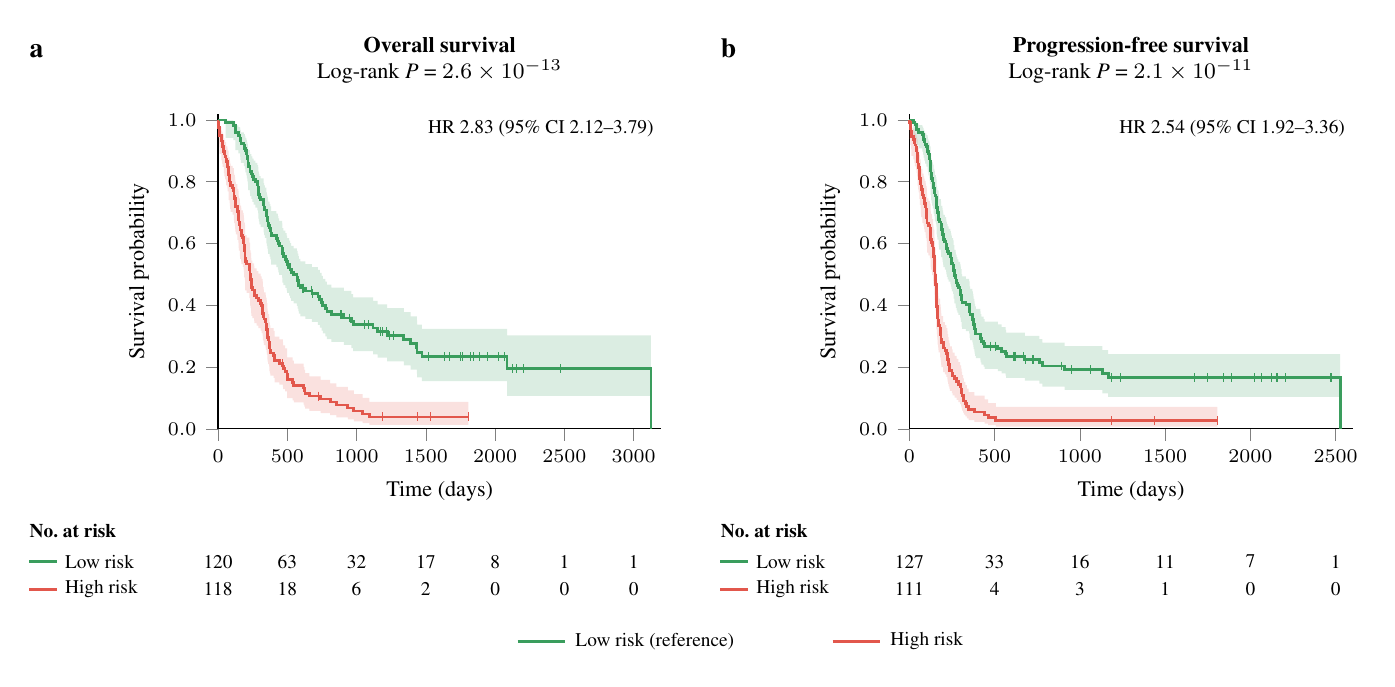
\begin{tikzpicture}
\begin{groupplot}[kmaxis, group style={group size=2 by 1, horizontal sep=31.5mm, vertical sep=42mm}]
\nextgroupplot[xmax=3200, xtick={0,500,1000,1500,2000,2500,3000}, title={\textbf{Overall survival}\\ Log-rank \textit{P} = $2.6\times10^{-13}$}]
\addplot[draw=none, fill=kmlow, fill opacity=0.18, forget plot] coordinates {(0.0,1.0000) (55.0,1.0000) (55.0,0.9988) (110.0,0.9988) (110.0,0.9958) (125.0,0.9958) (125.0,0.9874) (126.0,0.9874) (126.0,0.9824) (146.0,0.9824) (146.0,0.9772) (159.0,0.9772) (159.0,0.9718) (161.0,0.9718) (161.0,0.9661) (165.0,0.9661) (165.0,0.9603) (187.0,0.9603) (187.0,0.9543) (193.0,0.9543) (193.0,0.9482) (197.0,0.9482) (197.0,0.9419) (204.0,0.9419) (204.0,0.9356) (209.0,0.9356) (209.0,0.9292) (211.0,0.9292) (211.0,0.9227) (216.0,0.9227) (216.0,0.9161) (217.0,0.9161) (217.0,0.9094) (218.0,0.9094) (218.0,0.9027) (230.0,0.9027) (230.0,0.8959) (231.0,0.8959) (231.0,0.8891) (241.0,0.8891) (241.0,0.8822) (247.0,0.8822) (247.0,0.8752) (257.0,0.8752) (257.0,0.8682) (269.0,0.8682) (269.0,0.8612) (284.0,0.8612) (284.0,0.8541) (289.0,0.8541) (289.0,0.8470) (291.0,0.8470) (291.0,0.8398) (292.0,0.8398) (292.0,0.8326) (294.0,0.8326) (294.0,0.8253) (299.0,0.8253) (299.0,0.8180) (307.0,0.8180) (307.0,0.8107) (329.0,0.8107) (329.0,0.8033) (330.0,0.8033) (330.0,0.7959) (332.0,0.7959) (332.0,0.7885) (338.0,0.7885) (338.0,0.7810) (349.0,0.7810) (349.0,0.7660) (353.0,0.7660) (353.0,0.7584) (356.0,0.7584) (356.0,0.7508) (360.0,0.7508) (360.0,0.7432) (362.0,0.7432) (362.0,0.7356) (373.0,0.7356) (373.0,0.7279) (377.0,0.7279) (377.0,0.7202) (383.0,0.7202) (383.0,0.7125) (384.0,0.7125) (384.0,0.7047) (422.0,0.7047) (422.0,0.6969) (432.0,0.6969) (432.0,0.6891) (436.0,0.6891) (436.0,0.6813) (441.0,0.6813) (441.0,0.6734) (462.0,0.6734) (462.0,0.6655) (464.0,0.6655) (464.0,0.6576) (465.0,0.6576) (465.0,0.6497) (471.0,0.6497) (471.0,0.6418) (478.0,0.6418) (478.0,0.6418) (486.0,0.6418) (486.0,0.6337) (496.0,0.6337) (496.0,0.6256) (499.0,0.6256) (499.0,0.6174) (505.0,0.6174) (505.0,0.6174) (514.0,0.6174) (514.0,0.6092) (520.0,0.6092) (520.0,0.6009) (528.0,0.6009) (528.0,0.5926) (546.0,0.5926) (546.0,0.5842) (570.0,0.5842) (570.0,0.5759) (575.0,0.5759) (575.0,0.5675) (580.0,0.5675) (580.0,0.5590) (583.0,0.5590) (583.0,0.5506) (595.0,0.5506) (595.0,0.5421) (609.0,0.5421) (609.0,0.5421) (619.0,0.5421) (619.0,0.5421) (620.0,0.5421) (620.0,0.5421) (630.0,0.5421) (630.0,0.5332) (672.0,0.5332) (672.0,0.5332) (674.0,0.5332) (674.0,0.5332) (678.0,0.5332) (678.0,0.5239) (680.0,0.5239) (680.0,0.5239) (721.0,0.5239) (721.0,0.5145) (735.0,0.5145) (735.0,0.5050) (747.0,0.5050) (747.0,0.4954) (756.0,0.4954) (756.0,0.4858) (774.0,0.4858) (774.0,0.4762) (786.0,0.4762) (786.0,0.4665) (818.0,0.4665) (818.0,0.4568) (882.0,0.4568) (882.0,0.4568) (893.0,0.4568) (893.0,0.4568) (908.0,0.4568) (908.0,0.4466) (949.0,0.4466) (949.0,0.4466) (962.0,0.4466) (962.0,0.4361) (976.0,0.4361) (976.0,0.4256) (1060.0,0.4256) (1060.0,0.4256) (1086.0,0.4256) (1086.0,0.4256) (1119.0,0.4256) (1119.0,0.4145) (1152.0,0.4145) (1152.0,0.4033) (1173.0,0.4033) (1173.0,0.4033) (1184.0,0.4033) (1184.0,0.4033) (1214.0,0.4033) (1214.0,0.4033) (1221.0,0.4033) (1221.0,0.3910) (1239.0,0.3910) (1239.0,0.3910) (1267.0,0.3910) (1267.0,0.3910) (1341.0,0.3910) (1341.0,0.3778) (1390.0,0.3778) (1390.0,0.3644) (1435.0,0.3644) (1435.0,0.3509) (1437.0,0.3509) (1437.0,0.3372) (1472.0,0.3372) (1472.0,0.3233) (1519.0,0.3233) (1519.0,0.3233) (1633.0,0.3233) (1633.0,0.3233) (1673.0,0.3233) (1673.0,0.3233) (1750.0,0.3233) (1750.0,0.3233) (1767.0,0.3233) (1767.0,0.3233) (1821.0,0.3233) (1821.0,0.3233) (1843.0,0.3233) (1843.0,0.3233) (1890.0,0.3233) (1890.0,0.3233) (1948.0,0.3233) (1948.0,0.3233) (2024.0,0.3233) (2024.0,0.3233) (2066.0,0.3233) (2066.0,0.3233) (2086.0,0.3233) (2086.0,0.3025) (2123.0,0.3025) (2123.0,0.3025) (2156.0,0.3025) (2156.0,0.3025) (2205.0,0.3025) (2205.0,0.3025) (2473.0,0.3025) (2473.0,0.3025) (3125.0,0.3025) (3125.0,0.0000) (3125.0,0.0000) (3125.0,0.0000) (3125.0,0.0000) (3125.0,0.1067) (2473.0,0.1067) (2473.0,0.1067) (2205.0,0.1067) (2205.0,0.1067) (2156.0,0.1067) (2156.0,0.1067) (2123.0,0.1067) (2123.0,0.1067) (2086.0,0.1067) (2086.0,0.1540) (2066.0,0.1540) (2066.0,0.1540) (2024.0,0.1540) (2024.0,0.1540) (1948.0,0.1540) (1948.0,0.1540) (1890.0,0.1540) (1890.0,0.1540) (1843.0,0.1540) (1843.0,0.1540) (1821.0,0.1540) (1821.0,0.1540) (1767.0,0.1540) (1767.0,0.1540) (1750.0,0.1540) (1750.0,0.1540) (1673.0,0.1540) (1673.0,0.1540) (1633.0,0.1540) (1633.0,0.1540) (1519.0,0.1540) (1519.0,0.1540) (1472.0,0.1540) (1472.0,0.1664) (1437.0,0.1664) (1437.0,0.1790) (1435.0,0.1790) (1435.0,0.1919) (1390.0,0.1919) (1390.0,0.2050) (1341.0,0.2050) (1341.0,0.2183) (1267.0,0.2183) (1267.0,0.2183) (1239.0,0.2183) (1239.0,0.2183) (1221.0,0.2183) (1221.0,0.2303) (1214.0,0.2303) (1214.0,0.2303) (1184.0,0.2303) (1184.0,0.2303) (1173.0,0.2303) (1173.0,0.2303) (1152.0,0.2303) (1152.0,0.2409) (1119.0,0.2409) (1119.0,0.2516) (1086.0,0.2516) (1086.0,0.2516) (1060.0,0.2516) (1060.0,0.2516) (976.0,0.2516) (976.0,0.2615) (962.0,0.2615) (962.0,0.2715) (949.0,0.2715) (949.0,0.2715) (908.0,0.2715) (908.0,0.2812) (893.0,0.2812) (893.0,0.2812) (882.0,0.2812) (882.0,0.2812) (818.0,0.2812) (818.0,0.2904) (786.0,0.2904) (786.0,0.2996) (774.0,0.2996) (774.0,0.3089) (756.0,0.3089) (756.0,0.3182) (747.0,0.3182) (747.0,0.3275) (735.0,0.3275) (735.0,0.3369) (721.0,0.3369) (721.0,0.3464) (680.0,0.3464) (680.0,0.3464) (678.0,0.3464) (678.0,0.3556) (674.0,0.3556) (674.0,0.3556) (672.0,0.3556) (672.0,0.3556) (630.0,0.3556) (630.0,0.3644) (620.0,0.3644) (620.0,0.3644) (619.0,0.3644) (619.0,0.3644) (609.0,0.3644) (609.0,0.3644) (595.0,0.3644) (595.0,0.3727) (583.0,0.3727) (583.0,0.3810) (580.0,0.3810) (580.0,0.3893) (575.0,0.3893) (575.0,0.3977) (570.0,0.3977) (570.0,0.4060) (546.0,0.4060) (546.0,0.4144) (528.0,0.4144) (528.0,0.4229) (520.0,0.4229) (520.0,0.4313) (514.0,0.4313) (514.0,0.4398) (505.0,0.4398) (505.0,0.4398) (499.0,0.4398) (499.0,0.4482) (496.0,0.4482) (496.0,0.4566) (486.0,0.4566) (486.0,0.4650) (478.0,0.4650) (478.0,0.4650) (471.0,0.4650) (471.0,0.4733) (465.0,0.4733) (465.0,0.4816) (464.0,0.4816) (464.0,0.4899) (462.0,0.4899) (462.0,0.4983) (441.0,0.4983) (441.0,0.5066) (436.0,0.5066) (436.0,0.5151) (432.0,0.5151) (432.0,0.5235) (422.0,0.5235) (422.0,0.5320) (384.0,0.5320) (384.0,0.5404) (383.0,0.5404) (383.0,0.5490) (377.0,0.5490) (377.0,0.5575) (373.0,0.5575) (373.0,0.5661) (362.0,0.5661) (362.0,0.5747) (360.0,0.5747) (360.0,0.5833) (356.0,0.5833) (356.0,0.5920) (353.0,0.5920) (353.0,0.6007) (349.0,0.6007) (349.0,0.6181) (338.0,0.6181) (338.0,0.6269) (332.0,0.6269) (332.0,0.6357) (330.0,0.6357) (330.0,0.6446) (329.0,0.6446) (329.0,0.6534) (307.0,0.6534) (307.0,0.6623) (299.0,0.6623) (299.0,0.6713) (294.0,0.6713) (294.0,0.6803) (292.0,0.6803) (292.0,0.6893) (291.0,0.6893) (291.0,0.6984) (289.0,0.6984) (289.0,0.7075) (284.0,0.7075) (284.0,0.7166) (269.0,0.7166) (269.0,0.7258) (257.0,0.7258) (257.0,0.7351) (247.0,0.7351) (247.0,0.7444) (241.0,0.7444) (241.0,0.7537) (231.0,0.7537) (231.0,0.7631) (230.0,0.7631) (230.0,0.7725) (218.0,0.7725) (218.0,0.7820) (217.0,0.7820) (217.0,0.7916) (216.0,0.7916) (216.0,0.8013) (211.0,0.8013) (211.0,0.8110) (209.0,0.8110) (209.0,0.8208) (204.0,0.8208) (204.0,0.8306) (197.0,0.8306) (197.0,0.8406) (193.0,0.8406) (193.0,0.8507) (187.0,0.8507) (187.0,0.8608) (165.0,0.8608) (165.0,0.8711) (161.0,0.8711) (161.0,0.8815) (159.0,0.8815) (159.0,0.8921) (146.0,0.8921) (146.0,0.9028) (126.0,0.9028) (126.0,0.9136) (125.0,0.9136) (125.0,0.9350) (110.0,0.9350) (110.0,0.9423) (55.0,0.9423) (55.0,1.0000) (0.0,1.0000)} -- cycle;
\addplot[draw=none, fill=kmhigh, fill opacity=0.18, forget plot] coordinates {(0.0,0.9988) (6.0,0.9988) (6.0,0.9917) (10.0,0.9917) (10.0,0.9871) (12.0,0.9871) (12.0,0.9768) (24.0,0.9768) (24.0,0.9655) (30.0,0.9655) (30.0,0.9596) (33.0,0.9596) (33.0,0.9535) (42.0,0.9535) (42.0,0.9409) (45.0,0.9409) (45.0,0.9345) (51.0,0.9345) (51.0,0.9280) (58.0,0.9280) (58.0,0.9213) (59.0,0.9213) (59.0,0.9146) (67.0,0.9146) (67.0,0.9079) (69.0,0.9079) (69.0,0.9010) (76.0,0.9010) (76.0,0.8801) (84.0,0.8801) (84.0,0.8731) (85.0,0.8731) (85.0,0.8659) (87.0,0.8659) (87.0,0.8587) (90.0,0.8587) (90.0,0.8515) (106.0,0.8515) (106.0,0.8443) (114.0,0.8443) (114.0,0.8369) (115.0,0.8369) (115.0,0.8296) (116.0,0.8296) (116.0,0.8222) (121.0,0.8222) (121.0,0.8148) (124.0,0.8148) (124.0,0.8073) (125.0,0.8073) (125.0,0.7998) (128.0,0.7998) (128.0,0.7923) (139.0,0.7923) (139.0,0.7847) (140.0,0.7847) (140.0,0.7771) (147.0,0.7771) (147.0,0.7695) (149.0,0.7695) (149.0,0.7541) (151.0,0.7541) (151.0,0.7464) (157.0,0.7464) (157.0,0.7386) (158.0,0.7386) (158.0,0.7308) (159.0,0.7308) (159.0,0.7230) (167.0,0.7230) (167.0,0.7152) (169.0,0.7152) (169.0,0.7073) (179.0,0.7073) (179.0,0.6994) (184.0,0.6994) (184.0,0.6915) (186.0,0.6915) (186.0,0.6835) (188.0,0.6835) (188.0,0.6755) (189.0,0.6755) (189.0,0.6675) (193.0,0.6675) (193.0,0.6595) (195.0,0.6595) (195.0,0.6353) (196.0,0.6353) (196.0,0.6271) (206.0,0.6271) (206.0,0.6190) (227.0,0.6190) (227.0,0.6026) (231.0,0.6026) (231.0,0.5861) (232.0,0.5861) (232.0,0.5778) (235.0,0.5778) (235.0,0.5695) (239.0,0.5695) (239.0,0.5528) (240.0,0.5528) (240.0,0.5444) (247.0,0.5444) (247.0,0.5360) (261.0,0.5360) (261.0,0.5276) (262.0,0.5276) (262.0,0.5191) (279.0,0.5191) (279.0,0.5107) (292.0,0.5107) (292.0,0.5022) (307.0,0.5022) (307.0,0.4936) (315.0,0.4936) (315.0,0.4851) (322.0,0.4851) (322.0,0.4765) (323.0,0.4765) (323.0,0.4592) (330.0,0.4592) (330.0,0.4506) (331.0,0.4506) (331.0,0.4419) (343.0,0.4419) (343.0,0.4332) (346.0,0.4332) (346.0,0.4244) (351.0,0.4244) (351.0,0.4156) (352.0,0.4156) (352.0,0.4068) (357.0,0.4068) (357.0,0.3891) (358.0,0.3891) (358.0,0.3802) (362.0,0.3802) (362.0,0.3713) (368.0,0.3713) (368.0,0.3623) (370.0,0.3623) (370.0,0.3443) (375.0,0.3443) (375.0,0.3353) (377.0,0.3353) (377.0,0.3262) (401.0,0.3262) (401.0,0.3170) (408.0,0.3170) (408.0,0.3078) (409.0,0.3078) (409.0,0.2986) (443.0,0.2986) (443.0,0.2894) (465.0,0.2894) (465.0,0.2894) (468.0,0.2894) (468.0,0.2798) (470.0,0.2798) (470.0,0.2701) (484.0,0.2701) (484.0,0.2604) (498.0,0.2604) (498.0,0.2506) (499.0,0.2506) (499.0,0.2309) (538.0,0.2309) (538.0,0.2209) (547.0,0.2209) (547.0,0.2109) (618.0,0.2109) (618.0,0.2008) (623.0,0.2008) (623.0,0.1906) (628.0,0.1906) (628.0,0.1803) (659.0,0.1803) (659.0,0.1699) (725.0,0.1699) (725.0,0.1699) (740.0,0.1699) (740.0,0.1587) (810.0,0.1587) (810.0,0.1474) (855.0,0.1474) (855.0,0.1359) (937.0,0.1359) (937.0,0.1242) (980.0,0.1242) (980.0,0.1123) (1044.0,0.1123) (1044.0,0.1000) (1092.0,0.1000) (1092.0,0.0875) (1184.0,0.0875) (1184.0,0.0875) (1439.0,0.0875) (1439.0,0.0875) (1536.0,0.0875) (1536.0,0.0875) (1807.0,0.0875) (1807.0,0.0875) (1807.0,0.0875) (1807.0,0.0129) (1807.0,0.0129) (1807.0,0.0129) (1536.0,0.0129) (1536.0,0.0129) (1439.0,0.0129) (1439.0,0.0129) (1184.0,0.0129) (1184.0,0.0129) (1092.0,0.0129) (1092.0,0.0184) (1044.0,0.0184) (1044.0,0.0243) (980.0,0.0243) (980.0,0.0306) (937.0,0.0306) (937.0,0.0371) (855.0,0.0371) (855.0,0.0440) (810.0,0.0440) (810.0,0.0510) (740.0,0.0510) (740.0,0.0582) (725.0,0.0582) (725.0,0.0582) (659.0,0.0582) (659.0,0.0649) (628.0,0.0649) (628.0,0.0716) (623.0,0.0716) (623.0,0.0784) (618.0,0.0784) (618.0,0.0853) (547.0,0.0853) (547.0,0.0923) (538.0,0.0923) (538.0,0.0994) (499.0,0.0994) (499.0,0.1138) (498.0,0.1138) (498.0,0.1211) (484.0,0.1211) (484.0,0.1285) (470.0,0.1285) (470.0,0.1359) (468.0,0.1359) (468.0,0.1434) (465.0,0.1434) (465.0,0.1434) (443.0,0.1434) (443.0,0.1506) (409.0,0.1506) (409.0,0.1578) (408.0,0.1578) (408.0,0.1651) (401.0,0.1651) (401.0,0.1724) (377.0,0.1724) (377.0,0.1798) (375.0,0.1798) (375.0,0.1871) (370.0,0.1871) (370.0,0.2020) (368.0,0.2020) (368.0,0.2095) (362.0,0.2095) (362.0,0.2171) (358.0,0.2171) (358.0,0.2246) (357.0,0.2246) (357.0,0.2399) (352.0,0.2399) (352.0,0.2475) (351.0,0.2475) (351.0,0.2552) (346.0,0.2552) (346.0,0.2630) (343.0,0.2630) (343.0,0.2707) (331.0,0.2707) (331.0,0.2785) (330.0,0.2785) (330.0,0.2863) (323.0,0.2863) (323.0,0.3021) (322.0,0.3021) (322.0,0.3100) (315.0,0.3100) (315.0,0.3179) (307.0,0.3179) (307.0,0.3259) (292.0,0.3259) (292.0,0.3338) (279.0,0.3338) (279.0,0.3418) (262.0,0.3418) (262.0,0.3499) (261.0,0.3499) (261.0,0.3580) (247.0,0.3580) (247.0,0.3660) (240.0,0.3660) (240.0,0.3742) (239.0,0.3742) (239.0,0.3905) (235.0,0.3905) (235.0,0.3987) (232.0,0.3987) (232.0,0.4069) (231.0,0.4069) (231.0,0.4234) (227.0,0.4234) (227.0,0.4400) (206.0,0.4400) (206.0,0.4484) (196.0,0.4484) (196.0,0.4567) (195.0,0.4567) (195.0,0.4820) (193.0,0.4820) (193.0,0.4905) (189.0,0.4905) (189.0,0.4990) (188.0,0.4990) (188.0,0.5075) (186.0,0.5075) (186.0,0.5161) (184.0,0.5161) (184.0,0.5247) (179.0,0.5247) (179.0,0.5333) (169.0,0.5333) (169.0,0.5419) (167.0,0.5419) (167.0,0.5506) (159.0,0.5506) (159.0,0.5593) (158.0,0.5593) (158.0,0.5680) (157.0,0.5680) (157.0,0.5768) (151.0,0.5768) (151.0,0.5855) (149.0,0.5855) (149.0,0.6032) (147.0,0.6032) (147.0,0.6121) (140.0,0.6121) (140.0,0.6210) (139.0,0.6210) (139.0,0.6299) (128.0,0.6299) (128.0,0.6389) (125.0,0.6389) (125.0,0.6479) (124.0,0.6479) (124.0,0.6570) (121.0,0.6570) (121.0,0.6661) (116.0,0.6661) (116.0,0.6752) (115.0,0.6752) (115.0,0.6844) (114.0,0.6844) (114.0,0.6936) (106.0,0.6936) (106.0,0.7028) (90.0,0.7028) (90.0,0.7121) (87.0,0.7121) (87.0,0.7214) (85.0,0.7214) (85.0,0.7308) (84.0,0.7308) (84.0,0.7402) (76.0,0.7402) (76.0,0.7689) (69.0,0.7689) (69.0,0.7785) (67.0,0.7785) (67.0,0.7882) (59.0,0.7882) (59.0,0.7980) (58.0,0.7980) (58.0,0.8079) (51.0,0.8079) (51.0,0.8178) (45.0,0.8178) (45.0,0.8279) (42.0,0.8279) (42.0,0.8482) (33.0,0.8482) (33.0,0.8586) (30.0,0.8586) (30.0,0.8690) (24.0,0.8690) (24.0,0.8903) (12.0,0.8903) (12.0,0.9122) (10.0,0.9122) (10.0,0.9233) (6.0,0.9233) (6.0,0.9414) (0.0,0.9414)} -- cycle;
\addplot[const plot, kmlowline, forget plot] coordinates {(0.0,1.0000) (0.0,1.0000) (55.0,0.9917) (110.0,0.9833) (125.0,0.9667) (126.0,0.9583) (146.0,0.9500) (159.0,0.9417) (161.0,0.9333) (165.0,0.9250) (187.0,0.9167) (193.0,0.9083) (197.0,0.9000) (204.0,0.8917) (209.0,0.8833) (211.0,0.8750) (216.0,0.8667) (217.0,0.8583) (218.0,0.8500) (230.0,0.8417) (231.0,0.8333) (241.0,0.8250) (247.0,0.8167) (257.0,0.8083) (269.0,0.8000) (284.0,0.7917) (289.0,0.7833) (291.0,0.7750) (292.0,0.7667) (294.0,0.7583) (299.0,0.7500) (307.0,0.7417) (329.0,0.7333) (330.0,0.7250) (332.0,0.7167) (338.0,0.7083) (349.0,0.6917) (353.0,0.6833) (356.0,0.6750) (360.0,0.6667) (362.0,0.6583) (373.0,0.6500) (377.0,0.6417) (383.0,0.6333) (384.0,0.6250) (422.0,0.6167) (432.0,0.6083) (436.0,0.6000) (441.0,0.5917) (462.0,0.5833) (464.0,0.5750) (465.0,0.5667) (471.0,0.5583) (478.0,0.5583) (486.0,0.5499) (496.0,0.5414) (499.0,0.5330) (505.0,0.5330) (514.0,0.5244) (520.0,0.5158) (528.0,0.5072) (546.0,0.4986) (570.0,0.4900) (575.0,0.4814) (580.0,0.4728) (583.0,0.4642) (595.0,0.4556) (609.0,0.4556) (619.0,0.4556) (620.0,0.4556) (630.0,0.4465) (672.0,0.4465) (674.0,0.4465) (678.0,0.4370) (680.0,0.4370) (721.0,0.4273) (735.0,0.4176) (747.0,0.4078) (756.0,0.3981) (774.0,0.3884) (786.0,0.3787) (818.0,0.3690) (882.0,0.3690) (893.0,0.3690) (908.0,0.3588) (949.0,0.3588) (962.0,0.3482) (976.0,0.3377) (1060.0,0.3377) (1086.0,0.3377) (1119.0,0.3264) (1152.0,0.3151) (1173.0,0.3151) (1184.0,0.3151) (1214.0,0.3151) (1221.0,0.3025) (1239.0,0.3025) (1267.0,0.3025) (1341.0,0.2888) (1390.0,0.2750) (1435.0,0.2613) (1437.0,0.2475) (1472.0,0.2338) (1519.0,0.2338) (1633.0,0.2338) (1673.0,0.2338) (1750.0,0.2338) (1767.0,0.2338) (1821.0,0.2338) (1843.0,0.2338) (1890.0,0.2338) (1948.0,0.2338) (2024.0,0.2338) (2066.0,0.2338) (2086.0,0.1948) (2123.0,0.1948) (2156.0,0.1948) (2205.0,0.1948) (2473.0,0.1948) (3125.0,0.0000) (3125.0,0.0000)};
\addplot[only marks, mark=|, mark size=1.6pt, kmlow, forget plot] coordinates {(893.0,0.3690) (1890.0,0.2338) (1673.0,0.2338) (1267.0,0.3025) (882.0,0.3690) (672.0,0.4465) (680.0,0.4370) (1750.0,0.2338) (2123.0,0.1948) (1060.0,0.3377) (1214.0,0.3151) (1821.0,0.2338) (1086.0,0.3377) (2473.0,0.1948) (505.0,0.5330) (1239.0,0.3025) (1173.0,0.3151) (1633.0,0.2338) (2156.0,0.1948) (1843.0,0.2338) (949.0,0.3588) (2066.0,0.2338) (674.0,0.4465) (478.0,0.5583) (2024.0,0.2338) (1767.0,0.2338) (2205.0,0.1948) (1519.0,0.2338) (1948.0,0.2338) (619.0,0.4556) (1184.0,0.3151) (609.0,0.4556) (620.0,0.4556)};
\addplot[const plot, kmhighline, forget plot] coordinates {(0.0,1.0000) (0.0,0.9915) (6.0,0.9746) (10.0,0.9661) (12.0,0.9492) (24.0,0.9322) (30.0,0.9237) (33.0,0.9153) (42.0,0.8983) (45.0,0.8898) (51.0,0.8814) (58.0,0.8729) (59.0,0.8644) (67.0,0.8559) (69.0,0.8475) (76.0,0.8220) (84.0,0.8136) (85.0,0.8051) (87.0,0.7966) (90.0,0.7881) (106.0,0.7797) (114.0,0.7712) (115.0,0.7627) (116.0,0.7542) (121.0,0.7458) (124.0,0.7373) (125.0,0.7288) (128.0,0.7203) (139.0,0.7119) (140.0,0.7034) (147.0,0.6949) (149.0,0.6780) (151.0,0.6695) (157.0,0.6610) (158.0,0.6525) (159.0,0.6441) (167.0,0.6356) (169.0,0.6271) (179.0,0.6186) (184.0,0.6102) (186.0,0.6017) (188.0,0.5932) (189.0,0.5847) (193.0,0.5763) (195.0,0.5508) (196.0,0.5424) (206.0,0.5339) (227.0,0.5169) (231.0,0.5000) (232.0,0.4915) (235.0,0.4831) (239.0,0.4661) (240.0,0.4576) (247.0,0.4492) (261.0,0.4407) (262.0,0.4322) (279.0,0.4237) (292.0,0.4153) (307.0,0.4068) (315.0,0.3983) (322.0,0.3898) (323.0,0.3729) (330.0,0.3644) (331.0,0.3559) (343.0,0.3475) (346.0,0.3390) (351.0,0.3305) (352.0,0.3220) (357.0,0.3051) (358.0,0.2966) (362.0,0.2881) (368.0,0.2797) (370.0,0.2627) (375.0,0.2542) (377.0,0.2458) (401.0,0.2373) (408.0,0.2288) (409.0,0.2203) (443.0,0.2119) (465.0,0.2119) (468.0,0.2030) (470.0,0.1942) (484.0,0.1854) (498.0,0.1766) (499.0,0.1589) (538.0,0.1501) (547.0,0.1412) (618.0,0.1324) (623.0,0.1236) (628.0,0.1148) (659.0,0.1059) (725.0,0.1059) (740.0,0.0963) (810.0,0.0867) (855.0,0.0770) (937.0,0.0674) (980.0,0.0578) (1044.0,0.0482) (1092.0,0.0385) (1184.0,0.0385) (1439.0,0.0385) (1536.0,0.0385) (1807.0,0.0385) (1807.0,0.0385)};
\addplot[only marks, mark=|, mark size=1.6pt, kmhigh, forget plot] coordinates {(1536.0,0.0385) (1807.0,0.0385) (1439.0,0.0385) (725.0,0.1059) (465.0,0.2119) (1184.0,0.0385)};
\node[anchor=north east, font=\kmsmall, inner sep=1pt] at (rel axis cs:0.99,0.99) {HR 2.83 (95\% CI 2.12--3.79)};
\node[anchor=south west, inner sep=0pt, font=\kmletter, xshift=-24mm, yshift=7mm] at (rel axis cs:0,1) {a};
\node[anchor=west, inner sep=0pt, font=\kmsmall\bfseries, xshift=-24mm] at (axis cs:0,-0.33) {No.\ at risk};
\draw[kmlowline] ([xshift=-24mm]axis cs:0,-0.43) -- ([xshift=-20.5mm]axis cs:0,-0.43);
\node[anchor=west, inner sep=0pt, font=\kmsmall, xshift=-19.5mm] at (axis cs:0,-0.43) {Low risk};
\node[font=\kmsmall] at (axis cs:0,-0.43) {120};
\node[font=\kmsmall] at (axis cs:500,-0.43) {63};
\node[font=\kmsmall] at (axis cs:1000,-0.43) {32};
\node[font=\kmsmall] at (axis cs:1500,-0.43) {17};
\node[font=\kmsmall] at (axis cs:2000,-0.43) {8};
\node[font=\kmsmall] at (axis cs:2500,-0.43) {1};
\node[font=\kmsmall] at (axis cs:3000,-0.43) {1};
\draw[kmhighline] ([xshift=-24mm]axis cs:0,-0.52) -- ([xshift=-20.5mm]axis cs:0,-0.52);
\node[anchor=west, inner sep=0pt, font=\kmsmall, xshift=-19.5mm] at (axis cs:0,-0.52) {High risk};
\node[font=\kmsmall] at (axis cs:0,-0.52) {118};
\node[font=\kmsmall] at (axis cs:500,-0.52) {18};
\node[font=\kmsmall] at (axis cs:1000,-0.52) {6};
\node[font=\kmsmall] at (axis cs:1500,-0.52) {2};
\node[font=\kmsmall] at (axis cs:2000,-0.52) {0};
\node[font=\kmsmall] at (axis cs:2500,-0.52) {0};
\node[font=\kmsmall] at (axis cs:3000,-0.52) {0};
\nextgroupplot[xmax=2600, xtick={0,500,1000,1500,2000,2500}, title={\textbf{Progression-free survival}\\ Log-rank \textit{P} = $2.1\times10^{-11}$}]
\addplot[draw=none, fill=kmlow, fill opacity=0.18, forget plot] coordinates {(0.0,1.0000) (24.0,1.0000) (24.0,0.9989) (33.0,0.9989) (33.0,0.9960) (41.0,0.9960) (41.0,0.9923) (42.0,0.9923) (42.0,0.9881) (55.0,0.9881) (55.0,0.9834) (77.0,0.9834) (77.0,0.9785) (81.0,0.9785) (81.0,0.9733) (84.0,0.9733) (84.0,0.9680) (88.0,0.9680) (88.0,0.9625) (92.0,0.9625) (92.0,0.9568) (100.0,0.9568) (100.0,0.9511) (107.0,0.9511) (107.0,0.9452) (108.0,0.9452) (108.0,0.9392) (112.0,0.9392) (112.0,0.9332) (117.0,0.9332) (117.0,0.9270) (119.0,0.9270) (119.0,0.9208) (121.0,0.9208) (121.0,0.9146) (124.0,0.9146) (124.0,0.9082) (125.0,0.9082) (125.0,0.8889) (127.0,0.8889) (127.0,0.8823) (128.0,0.8823) (128.0,0.8757) (130.0,0.8757) (130.0,0.8691) (134.0,0.8691) (134.0,0.8624) (138.0,0.8624) (138.0,0.8557) (142.0,0.8557) (142.0,0.8489) (143.0,0.8489) (143.0,0.8421) (146.0,0.8421) (146.0,0.8353) (149.0,0.8353) (149.0,0.8284) (150.0,0.8284) (150.0,0.8215) (156.0,0.8215) (156.0,0.8146) (159.0,0.8146) (159.0,0.8076) (160.0,0.8076) (160.0,0.7866) (163.0,0.7866) (163.0,0.7795) (164.0,0.7795) (164.0,0.7724) (171.0,0.7724) (171.0,0.7652) (172.0,0.7652) (172.0,0.7581) (173.0,0.7581) (173.0,0.7509) (175.0,0.7509) (175.0,0.7437) (185.0,0.7437) (185.0,0.7364) (187.0,0.7364) (187.0,0.7219) (193.0,0.7219) (193.0,0.7146) (195.0,0.7146) (195.0,0.7073) (198.0,0.7073) (198.0,0.6999) (200.0,0.6999) (200.0,0.6925) (208.0,0.6925) (208.0,0.6851) (215.0,0.6851) (215.0,0.6777) (217.0,0.6777) (217.0,0.6703) (220.0,0.6703) (220.0,0.6628) (225.0,0.6628) (225.0,0.6553) (230.0,0.6553) (230.0,0.6478) (241.0,0.6478) (241.0,0.6403) (244.0,0.6403) (244.0,0.6327) (247.0,0.6327) (247.0,0.6252) (249.0,0.6252) (249.0,0.6176) (256.0,0.6176) (256.0,0.6099) (260.0,0.6099) (260.0,0.5947) (264.0,0.5947) (264.0,0.5793) (271.0,0.5793) (271.0,0.5716) (273.0,0.5716) (273.0,0.5638) (277.0,0.5638) (277.0,0.5561) (282.0,0.5561) (282.0,0.5483) (287.0,0.5483) (287.0,0.5405) (297.0,0.5405) (297.0,0.5327) (300.0,0.5327) (300.0,0.5248) (302.0,0.5248) (302.0,0.5170) (307.0,0.5170) (307.0,0.5012) (309.0,0.5012) (309.0,0.4933) (332.0,0.4933) (332.0,0.4853) (351.0,0.4853) (351.0,0.4774) (353.0,0.4774) (353.0,0.4694) (354.0,0.4694) (354.0,0.4613) (356.0,0.4613) (356.0,0.4533) (370.0,0.4533) (370.0,0.4453) (372.0,0.4453) (372.0,0.4372) (376.0,0.4372) (376.0,0.4291) (377.0,0.4291) (377.0,0.4209) (381.0,0.4209) (381.0,0.4128) (383.0,0.4128) (383.0,0.4046) (386.0,0.4046) (386.0,0.3964) (390.0,0.3964) (390.0,0.3882) (417.0,0.3882) (417.0,0.3799) (418.0,0.3799) (418.0,0.3717) (423.0,0.3717) (423.0,0.3634) (436.0,0.3634) (436.0,0.3550) (441.0,0.3550) (441.0,0.3467) (478.0,0.3467) (478.0,0.3467) (505.0,0.3467) (505.0,0.3467) (519.0,0.3467) (519.0,0.3378) (541.0,0.3378) (541.0,0.3290) (565.0,0.3290) (565.0,0.3201) (568.0,0.3201) (568.0,0.3112) (609.0,0.3112) (609.0,0.3112) (619.0,0.3112) (619.0,0.3112) (620.0,0.3112) (620.0,0.3112) (672.0,0.3112) (672.0,0.3112) (678.0,0.3112) (678.0,0.3011) (680.0,0.3011) (680.0,0.3011) (725.0,0.3011) (725.0,0.3011) (763.0,0.3011) (763.0,0.2902) (780.0,0.2902) (780.0,0.2792) (893.0,0.2792) (893.0,0.2792) (910.0,0.2792) (910.0,0.2677) (949.0,0.2677) (949.0,0.2677) (1060.0,0.2677) (1060.0,0.2677) (1132.0,0.2677) (1132.0,0.2550) (1166.0,0.2550) (1166.0,0.2421) (1184.0,0.2421) (1184.0,0.2421) (1239.0,0.2421) (1239.0,0.2421) (1673.0,0.2421) (1673.0,0.2421) (1750.0,0.2421) (1750.0,0.2421) (1843.0,0.2421) (1843.0,0.2421) (1890.0,0.2421) (1890.0,0.2421) (2024.0,0.2421) (2024.0,0.2421) (2066.0,0.2421) (2066.0,0.2421) (2123.0,0.2421) (2123.0,0.2421) (2156.0,0.2421) (2156.0,0.2421) (2205.0,0.2421) (2205.0,0.2421) (2473.0,0.2421) (2473.0,0.2421) (2527.0,0.2421) (2527.0,0.0000) (2527.0,0.0000) (2527.0,0.0000) (2527.0,0.0000) (2527.0,0.1033) (2473.0,0.1033) (2473.0,0.1033) (2205.0,0.1033) (2205.0,0.1033) (2156.0,0.1033) (2156.0,0.1033) (2123.0,0.1033) (2123.0,0.1033) (2066.0,0.1033) (2066.0,0.1033) (2024.0,0.1033) (2024.0,0.1033) (1890.0,0.1033) (1890.0,0.1033) (1843.0,0.1033) (1843.0,0.1033) (1750.0,0.1033) (1750.0,0.1033) (1673.0,0.1033) (1673.0,0.1033) (1239.0,0.1033) (1239.0,0.1033) (1184.0,0.1033) (1184.0,0.1033) (1166.0,0.1033) (1166.0,0.1147) (1132.0,0.1147) (1132.0,0.1263) (1060.0,0.1263) (1060.0,0.1263) (949.0,0.1263) (949.0,0.1263) (910.0,0.1263) (910.0,0.1365) (893.0,0.1365) (893.0,0.1365) (780.0,0.1365) (780.0,0.1461) (763.0,0.1461) (763.0,0.1558) (725.0,0.1558) (725.0,0.1558) (680.0,0.1558) (680.0,0.1558) (678.0,0.1558) (678.0,0.1646) (672.0,0.1646) (672.0,0.1646) (620.0,0.1646) (620.0,0.1646) (619.0,0.1646) (619.0,0.1646) (609.0,0.1646) (609.0,0.1646) (568.0,0.1646) (568.0,0.1719) (565.0,0.1719) (565.0,0.1793) (541.0,0.1793) (541.0,0.1867) (519.0,0.1867) (519.0,0.1941) (505.0,0.1941) (505.0,0.1941) (478.0,0.1941) (478.0,0.1941) (441.0,0.1941) (441.0,0.2011) (436.0,0.2011) (436.0,0.2081) (423.0,0.2081) (423.0,0.2151) (418.0,0.2151) (418.0,0.2221) (417.0,0.2221) (417.0,0.2292) (390.0,0.2292) (390.0,0.2363) (386.0,0.2363) (386.0,0.2435) (383.0,0.2435) (383.0,0.2506) (381.0,0.2506) (381.0,0.2578) (377.0,0.2578) (377.0,0.2650) (376.0,0.2650) (376.0,0.2723) (372.0,0.2723) (372.0,0.2795) (370.0,0.2795) (370.0,0.2868) (356.0,0.2868) (356.0,0.2941) (354.0,0.2941) (354.0,0.3015) (353.0,0.3015) (353.0,0.3088) (351.0,0.3088) (351.0,0.3162) (332.0,0.3162) (332.0,0.3236) (309.0,0.3236) (309.0,0.3310) (307.0,0.3310) (307.0,0.3459) (302.0,0.3459) (302.0,0.3534) (300.0,0.3534) (300.0,0.3609) (297.0,0.3609) (297.0,0.3685) (287.0,0.3685) (287.0,0.3760) (282.0,0.3760) (282.0,0.3836) (277.0,0.3836) (277.0,0.3912) (273.0,0.3912) (273.0,0.3988) (271.0,0.3988) (271.0,0.4065) (264.0,0.4065) (264.0,0.4218) (260.0,0.4218) (260.0,0.4373) (256.0,0.4373) (256.0,0.4450) (249.0,0.4450) (249.0,0.4528) (247.0,0.4528) (247.0,0.4606) (244.0,0.4606) (244.0,0.4684) (241.0,0.4684) (241.0,0.4762) (230.0,0.4762) (230.0,0.4841) (225.0,0.4841) (225.0,0.4920) (220.0,0.4920) (220.0,0.4999) (217.0,0.4999) (217.0,0.5078) (215.0,0.5078) (215.0,0.5158) (208.0,0.5158) (208.0,0.5237) (200.0,0.5237) (200.0,0.5317) (198.0,0.5317) (198.0,0.5397) (195.0,0.5397) (195.0,0.5478) (193.0,0.5478) (193.0,0.5558) (187.0,0.5558) (187.0,0.5720) (185.0,0.5720) (185.0,0.5802) (175.0,0.5802) (175.0,0.5883) (173.0,0.5883) (173.0,0.5965) (172.0,0.5965) (172.0,0.6047) (171.0,0.6047) (171.0,0.6130) (164.0,0.6130) (164.0,0.6212) (163.0,0.6212) (163.0,0.6295) (160.0,0.6295) (160.0,0.6546) (159.0,0.6546) (159.0,0.6630) (156.0,0.6630) (156.0,0.6714) (150.0,0.6714) (150.0,0.6799) (149.0,0.6799) (149.0,0.6884) (146.0,0.6884) (146.0,0.6969) (143.0,0.6969) (143.0,0.7055) (142.0,0.7055) (142.0,0.7141) (138.0,0.7141) (138.0,0.7228) (134.0,0.7228) (134.0,0.7314) (130.0,0.7314) (130.0,0.7402) (128.0,0.7402) (128.0,0.7490) (127.0,0.7490) (127.0,0.7578) (125.0,0.7578) (125.0,0.7845) (124.0,0.7845) (124.0,0.7935) (121.0,0.7935) (121.0,0.8026) (119.0,0.8026) (119.0,0.8118) (117.0,0.8118) (117.0,0.8210) (112.0,0.8210) (112.0,0.8303) (108.0,0.8303) (108.0,0.8396) (107.0,0.8396) (107.0,0.8491) (100.0,0.8491) (100.0,0.8586) (92.0,0.8586) (92.0,0.8682) (88.0,0.8682) (88.0,0.8780) (84.0,0.8780) (84.0,0.8879) (81.0,0.8879) (81.0,0.8979) (77.0,0.8979) (77.0,0.9080) (55.0,0.9080) (55.0,0.9183) (42.0,0.9183) (42.0,0.9286) (41.0,0.9286) (41.0,0.9385) (33.0,0.9385) (33.0,0.9454) (24.0,0.9454) (24.0,1.0000) (0.0,1.0000)} -- cycle;
\addplot[draw=none, fill=kmhigh, fill opacity=0.18, forget plot] coordinates {(0.0,0.9987) (6.0,0.9987) (6.0,0.9912) (10.0,0.9912) (10.0,0.9863) (12.0,0.9863) (12.0,0.9753) (24.0,0.9753) (24.0,0.9694) (30.0,0.9694) (30.0,0.9633) (33.0,0.9633) (33.0,0.9570) (39.0,0.9570) (39.0,0.9505) (42.0,0.9505) (42.0,0.9439) (45.0,0.9439) (45.0,0.9371) (48.0,0.9371) (48.0,0.9302) (49.0,0.9302) (49.0,0.9162) (51.0,0.9162) (51.0,0.9091) (54.0,0.9091) (54.0,0.9019) (58.0,0.9019) (58.0,0.8946) (59.0,0.8946) (59.0,0.8872) (61.0,0.8872) (61.0,0.8723) (66.0,0.8723) (66.0,0.8647) (67.0,0.8647) (67.0,0.8571) (68.0,0.8571) (68.0,0.8495) (69.0,0.8495) (69.0,0.8418) (76.0,0.8418) (76.0,0.8262) (84.0,0.8262) (84.0,0.8184) (87.0,0.8184) (87.0,0.8105) (90.0,0.8105) (90.0,0.8025) (95.0,0.8025) (95.0,0.7946) (97.0,0.7946) (97.0,0.7866) (101.0,0.7866) (101.0,0.7785) (102.0,0.7785) (102.0,0.7623) (104.0,0.7623) (104.0,0.7459) (111.0,0.7459) (111.0,0.7377) (121.0,0.7377) (121.0,0.7294) (124.0,0.7294) (124.0,0.7128) (125.0,0.7128) (125.0,0.7044) (126.0,0.7044) (126.0,0.6961) (132.0,0.6961) (132.0,0.6876) (134.0,0.6876) (134.0,0.6792) (139.0,0.6792) (139.0,0.6707) (140.0,0.6707) (140.0,0.6622) (141.0,0.6622) (141.0,0.6536) (143.0,0.6536) (143.0,0.6451) (146.0,0.6451) (146.0,0.6364) (147.0,0.6364) (147.0,0.6192) (148.0,0.6192) (148.0,0.6017) (150.0,0.6017) (150.0,0.5930) (151.0,0.5930) (151.0,0.5842) (154.0,0.5842) (154.0,0.5666) (155.0,0.5666) (155.0,0.5577) (157.0,0.5577) (157.0,0.5488) (158.0,0.5488) (158.0,0.5130) (159.0,0.5130) (159.0,0.5039) (161.0,0.5039) (161.0,0.4858) (163.0,0.4858) (163.0,0.4766) (164.0,0.4766) (164.0,0.4675) (166.0,0.4675) (166.0,0.4491) (168.0,0.4491) (168.0,0.4398) (170.0,0.4398) (170.0,0.4305) (172.0,0.4305) (172.0,0.4212) (180.0,0.4212) (180.0,0.4118) (181.0,0.4118) (181.0,0.4025) (183.0,0.4025) (183.0,0.3930) (185.0,0.3930) (185.0,0.3836) (186.0,0.3836) (186.0,0.3741) (188.0,0.3741) (188.0,0.3645) (198.0,0.3645) (198.0,0.3454) (209.0,0.3454) (209.0,0.3357) (217.0,0.3357) (217.0,0.3260) (223.0,0.3260) (223.0,0.3163) (224.0,0.3163) (224.0,0.3065) (228.0,0.3065) (228.0,0.2966) (230.0,0.2966) (230.0,0.2867) (235.0,0.2867) (235.0,0.2768) (237.0,0.2768) (237.0,0.2668) (250.0,0.2668) (250.0,0.2568) (254.0,0.2568) (254.0,0.2467) (265.0,0.2467) (265.0,0.2365) (277.0,0.2365) (277.0,0.2262) (288.0,0.2262) (288.0,0.2159) (298.0,0.2159) (298.0,0.2055) (303.0,0.2055) (303.0,0.1951) (306.0,0.1951) (306.0,0.1845) (309.0,0.1845) (309.0,0.1738) (316.0,0.1738) (316.0,0.1631) (319.0,0.1631) (319.0,0.1522) (329.0,0.1522) (329.0,0.1411) (337.0,0.1411) (337.0,0.1300) (348.0,0.1300) (348.0,0.1186) (381.0,0.1186) (381.0,0.1070) (442.0,0.1070) (442.0,0.0952) (462.0,0.0952) (462.0,0.0831) (507.0,0.0831) (507.0,0.0706) (1184.0,0.0706) (1184.0,0.0706) (1439.0,0.0706) (1439.0,0.0706) (1807.0,0.0706) (1807.0,0.0706) (1807.0,0.0706) (1807.0,0.0073) (1807.0,0.0073) (1807.0,0.0073) (1439.0,0.0073) (1439.0,0.0073) (1184.0,0.0073) (1184.0,0.0073) (507.0,0.0073) (507.0,0.0118) (462.0,0.0118) (462.0,0.0168) (442.0,0.0168) (442.0,0.0222) (381.0,0.0222) (381.0,0.0278) (348.0,0.0278) (348.0,0.0337) (337.0,0.0337) (337.0,0.0398) (329.0,0.0398) (329.0,0.0461) (319.0,0.0461) (319.0,0.0525) (316.0,0.0525) (316.0,0.0591) (309.0,0.0591) (309.0,0.0658) (306.0,0.0658) (306.0,0.0726) (303.0,0.0726) (303.0,0.0795) (298.0,0.0795) (298.0,0.0865) (288.0,0.0865) (288.0,0.0936) (277.0,0.0936) (277.0,0.1007) (265.0,0.1007) (265.0,0.1080) (254.0,0.1080) (254.0,0.1153) (250.0,0.1153) (250.0,0.1227) (237.0,0.1227) (237.0,0.1301) (235.0,0.1301) (235.0,0.1376) (230.0,0.1376) (230.0,0.1452) (228.0,0.1452) (228.0,0.1528) (224.0,0.1528) (224.0,0.1604) (223.0,0.1604) (223.0,0.1681) (217.0,0.1681) (217.0,0.1759) (209.0,0.1759) (209.0,0.1837) (198.0,0.1837) (198.0,0.1994) (188.0,0.1994) (188.0,0.2074) (186.0,0.2074) (186.0,0.2153) (185.0,0.2153) (185.0,0.2233) (183.0,0.2233) (183.0,0.2314) (181.0,0.2314) (181.0,0.2395) (180.0,0.2395) (180.0,0.2476) (172.0,0.2476) (172.0,0.2558) (170.0,0.2558) (170.0,0.2640) (168.0,0.2640) (168.0,0.2722) (166.0,0.2722) (166.0,0.2888) (164.0,0.2888) (164.0,0.2971) (163.0,0.2971) (163.0,0.3055) (161.0,0.3055) (161.0,0.3223) (159.0,0.3223) (159.0,0.3308) (158.0,0.3308) (158.0,0.3649) (157.0,0.3649) (157.0,0.3735) (155.0,0.3735) (155.0,0.3822) (154.0,0.3822) (154.0,0.3996) (151.0,0.3996) (151.0,0.4083) (150.0,0.4083) (150.0,0.4171) (148.0,0.4171) (148.0,0.4347) (147.0,0.4347) (147.0,0.4524) (146.0,0.4524) (146.0,0.4613) (143.0,0.4613) (143.0,0.4703) (141.0,0.4703) (141.0,0.4792) (140.0,0.4792) (140.0,0.4882) (139.0,0.4882) (139.0,0.4973) (134.0,0.4973) (134.0,0.5064) (132.0,0.5064) (132.0,0.5155) (126.0,0.5155) (126.0,0.5246) (125.0,0.5246) (125.0,0.5337) (124.0,0.5337) (124.0,0.5522) (121.0,0.5522) (121.0,0.5614) (111.0,0.5614) (111.0,0.5707) (104.0,0.5707) (104.0,0.5894) (102.0,0.5894) (102.0,0.6083) (101.0,0.6083) (101.0,0.6177) (97.0,0.6177) (97.0,0.6272) (95.0,0.6272) (95.0,0.6368) (90.0,0.6368) (90.0,0.6464) (87.0,0.6464) (87.0,0.6560) (84.0,0.6560) (84.0,0.6657) (76.0,0.6657) (76.0,0.6852) (69.0,0.6852) (69.0,0.6950) (68.0,0.6950) (68.0,0.7049) (67.0,0.7049) (67.0,0.7148) (66.0,0.7148) (66.0,0.7248) (61.0,0.7248) (61.0,0.7449) (59.0,0.7449) (59.0,0.7550) (58.0,0.7550) (58.0,0.7653) (54.0,0.7653) (54.0,0.7755) (51.0,0.7755) (51.0,0.7859) (49.0,0.7859) (49.0,0.8069) (48.0,0.8069) (48.0,0.8175) (45.0,0.8175) (45.0,0.8282) (42.0,0.8282) (42.0,0.8390) (39.0,0.8390) (39.0,0.8500) (33.0,0.8500) (33.0,0.8611) (30.0,0.8611) (30.0,0.8723) (24.0,0.8723) (24.0,0.8836) (12.0,0.8836) (12.0,0.9068) (10.0,0.9068) (10.0,0.9186) (6.0,0.9186) (6.0,0.9378) (0.0,0.9378)} -- cycle;
\addplot[const plot, kmlowline, forget plot] coordinates {(0.0,1.0000) (0.0,1.0000) (24.0,0.9921) (33.0,0.9843) (41.0,0.9764) (42.0,0.9685) (55.0,0.9606) (77.0,0.9528) (81.0,0.9449) (84.0,0.9370) (88.0,0.9291) (92.0,0.9213) (100.0,0.9134) (107.0,0.9055) (108.0,0.8976) (112.0,0.8898) (117.0,0.8819) (119.0,0.8740) (121.0,0.8661) (124.0,0.8583) (125.0,0.8346) (127.0,0.8268) (128.0,0.8189) (130.0,0.8110) (134.0,0.8031) (138.0,0.7953) (142.0,0.7874) (143.0,0.7795) (146.0,0.7717) (149.0,0.7638) (150.0,0.7559) (156.0,0.7480) (159.0,0.7402) (160.0,0.7165) (163.0,0.7087) (164.0,0.7008) (171.0,0.6929) (172.0,0.6850) (173.0,0.6772) (175.0,0.6693) (185.0,0.6614) (187.0,0.6457) (193.0,0.6378) (195.0,0.6299) (198.0,0.6220) (200.0,0.6142) (208.0,0.6063) (215.0,0.5984) (217.0,0.5906) (220.0,0.5827) (225.0,0.5748) (230.0,0.5669) (241.0,0.5591) (244.0,0.5512) (247.0,0.5433) (249.0,0.5354) (256.0,0.5276) (260.0,0.5118) (264.0,0.4961) (271.0,0.4882) (273.0,0.4803) (277.0,0.4724) (282.0,0.4646) (287.0,0.4567) (297.0,0.4488) (300.0,0.4409) (302.0,0.4331) (307.0,0.4173) (309.0,0.4094) (332.0,0.4016) (351.0,0.3937) (353.0,0.3858) (354.0,0.3780) (356.0,0.3701) (370.0,0.3622) (372.0,0.3543) (376.0,0.3465) (377.0,0.3386) (381.0,0.3307) (383.0,0.3228) (386.0,0.3150) (390.0,0.3071) (417.0,0.2992) (418.0,0.2913) (423.0,0.2835) (436.0,0.2756) (441.0,0.2677) (478.0,0.2677) (505.0,0.2677) (519.0,0.2594) (541.0,0.2510) (565.0,0.2426) (568.0,0.2343) (609.0,0.2343) (619.0,0.2343) (620.0,0.2343) (672.0,0.2343) (678.0,0.2245) (680.0,0.2245) (725.0,0.2245) (763.0,0.2138) (780.0,0.2031) (893.0,0.2031) (910.0,0.1918) (949.0,0.1918) (1060.0,0.1918) (1132.0,0.1790) (1166.0,0.1663) (1184.0,0.1663) (1239.0,0.1663) (1673.0,0.1663) (1750.0,0.1663) (1843.0,0.1663) (1890.0,0.1663) (2024.0,0.1663) (2066.0,0.1663) (2123.0,0.1663) (2156.0,0.1663) (2205.0,0.1663) (2473.0,0.1663) (2527.0,0.0000) (2527.0,0.0000)};
\addplot[only marks, mark=|, mark size=1.6pt, kmlow, forget plot] coordinates {(893.0,0.2031) (1890.0,0.1663) (1673.0,0.1663) (672.0,0.2343) (680.0,0.2245) (1750.0,0.1663) (2123.0,0.1663) (1060.0,0.1918) (2473.0,0.1663) (505.0,0.2677) (1239.0,0.1663) (2156.0,0.1663) (1843.0,0.1663) (949.0,0.1918) (2066.0,0.1663) (478.0,0.2677) (2024.0,0.1663) (2205.0,0.1663) (725.0,0.2245) (619.0,0.2343) (1184.0,0.1663) (609.0,0.2343) (620.0,0.2343)};
\addplot[const plot, kmhighline, forget plot] coordinates {(0.0,1.0000) (0.0,0.9910) (6.0,0.9730) (10.0,0.9640) (12.0,0.9459) (24.0,0.9369) (30.0,0.9279) (33.0,0.9189) (39.0,0.9099) (42.0,0.9009) (45.0,0.8919) (48.0,0.8829) (49.0,0.8649) (51.0,0.8559) (54.0,0.8468) (58.0,0.8378) (59.0,0.8288) (61.0,0.8108) (66.0,0.8018) (67.0,0.7928) (68.0,0.7838) (69.0,0.7748) (76.0,0.7568) (84.0,0.7477) (87.0,0.7387) (90.0,0.7297) (95.0,0.7207) (97.0,0.7117) (101.0,0.7027) (102.0,0.6847) (104.0,0.6667) (111.0,0.6577) (121.0,0.6486) (124.0,0.6306) (125.0,0.6216) (126.0,0.6126) (132.0,0.6036) (134.0,0.5946) (139.0,0.5856) (140.0,0.5766) (141.0,0.5676) (143.0,0.5586) (146.0,0.5495) (147.0,0.5315) (148.0,0.5135) (150.0,0.5045) (151.0,0.4955) (154.0,0.4775) (155.0,0.4685) (157.0,0.4595) (158.0,0.4234) (159.0,0.4144) (161.0,0.3964) (163.0,0.3874) (164.0,0.3784) (166.0,0.3604) (168.0,0.3514) (170.0,0.3423) (172.0,0.3333) (180.0,0.3243) (181.0,0.3153) (183.0,0.3063) (185.0,0.2973) (186.0,0.2883) (188.0,0.2793) (198.0,0.2613) (209.0,0.2523) (217.0,0.2432) (223.0,0.2342) (224.0,0.2252) (228.0,0.2162) (230.0,0.2072) (235.0,0.1982) (237.0,0.1892) (250.0,0.1802) (254.0,0.1712) (265.0,0.1622) (277.0,0.1532) (288.0,0.1441) (298.0,0.1351) (303.0,0.1261) (306.0,0.1171) (309.0,0.1081) (316.0,0.0991) (319.0,0.0901) (329.0,0.0811) (337.0,0.0721) (348.0,0.0631) (381.0,0.0541) (442.0,0.0450) (462.0,0.0360) (507.0,0.0270) (1184.0,0.0270) (1439.0,0.0270) (1807.0,0.0270) (1807.0,0.0270)};
\addplot[only marks, mark=|, mark size=1.6pt, kmhigh, forget plot] coordinates {(1807.0,0.0270) (1439.0,0.0270) (1184.0,0.0270)};
\node[anchor=north east, font=\kmsmall, inner sep=1pt] at (rel axis cs:0.99,0.99) {HR 2.54 (95\% CI 1.92--3.36)};
\node[anchor=south west, inner sep=0pt, font=\kmletter, xshift=-24mm, yshift=7mm] at (rel axis cs:0,1) {b};
\node[anchor=west, inner sep=0pt, font=\kmsmall\bfseries, xshift=-24mm] at (axis cs:0,-0.33) {No.\ at risk};
\draw[kmlowline] ([xshift=-24mm]axis cs:0,-0.43) -- ([xshift=-20.5mm]axis cs:0,-0.43);
\node[anchor=west, inner sep=0pt, font=\kmsmall, xshift=-19.5mm] at (axis cs:0,-0.43) {Low risk};
\node[font=\kmsmall] at (axis cs:0,-0.43) {127};
\node[font=\kmsmall] at (axis cs:500,-0.43) {33};
\node[font=\kmsmall] at (axis cs:1000,-0.43) {16};
\node[font=\kmsmall] at (axis cs:1500,-0.43) {11};
\node[font=\kmsmall] at (axis cs:2000,-0.43) {7};
\node[font=\kmsmall] at (axis cs:2500,-0.43) {1};
\draw[kmhighline] ([xshift=-24mm]axis cs:0,-0.52) -- ([xshift=-20.5mm]axis cs:0,-0.52);
\node[anchor=west, inner sep=0pt, font=\kmsmall, xshift=-19.5mm] at (axis cs:0,-0.52) {High risk};
\node[font=\kmsmall] at (axis cs:0,-0.52) {111};
\node[font=\kmsmall] at (axis cs:500,-0.52) {4};
\node[font=\kmsmall] at (axis cs:1000,-0.52) {3};
\node[font=\kmsmall] at (axis cs:1500,-0.52) {1};
\node[font=\kmsmall] at (axis cs:2000,-0.52) {0};
\node[font=\kmsmall] at (axis cs:2500,-0.52) {0};
\end{groupplot}
\coordinate (kmleg) at ($(group c1r1.south)!0.5!(group c2r1.south)$);
\draw[kmlowline] ([xshift=-34mm,yshift=-27mm]kmleg) -- ++(6mm,0) node[right, font=\kmsmall, text=black] {Low risk (reference)};
\draw[kmhighline] ([xshift=6mm,yshift=-27mm]kmleg) -- ++(6mm,0) node[right, font=\kmsmall, text=black] {High risk};
\end{tikzpicture}
\end{adjustbox}
\caption{Kaplan--Meier curves of (a) overall and (b) progression-free survival by the risk group of the proposed model. In each outer fold of nested cross-validation, test patients with a risk score above the median of the outer training patients were classified as high risk, and the five test folds were pooled (n = 238; not an independent test set). Shaded bands, 95\% CI; tick marks, censored patients; HR, high versus low risk (reference) from a univariable Cox model; \textit{P}, log-rank test. CI = confidence interval, HR = hazard ratio}
\label{fig:km_overall}
\end{figure}

% ===== 3.6 Subgroup analysis (nested CV) =====
\begin{table}[htbp]
\centering
\setlength{\belowcaptionskip}{4pt}
\caption{Performance of the Proposed Model in Clinical Subgroups}
\label{tab:subgroups}
\footnotesize\setlength{\tabcolsep}{2.5pt}
\begin{adjustbox}{max width=\textwidth}
\begin{tabular}{@{}lc ccc ccc@{}}
\toprule
Subgroup & Patients & \multicolumn{3}{c}{OS} & \multicolumn{3}{c}{PFS} \\
\cmidrule(lr){3-5}\cmidrule(l){6-8}
 & & C-index (95\% CI) & HR (95\% CI) & \textit{P}\textsubscript{int} & C-index (95\% CI) & HR (95\% CI) & \textit{P}\textsubscript{int} \\
\midrule
All patients & 238 & 0.724 (0.685--0.762) & 2.83 (2.12--3.79) & & 0.672 (0.632--0.710) & 2.54 (1.92--3.36) & \\
\addlinespace
Age & & & & 0.747 & & & 0.023 \\
\quad $<$ 70 years & 111 & 0.699 (0.626--0.764) & 2.73 (1.78--4.20) & & 0.626 (0.553--0.699) & 1.84 (1.22--2.77) & \\
\quad $\geq$ 70 years & 127 & 0.738 (0.681--0.789) & 2.69 (1.81--4.01) & & 0.709 (0.649--0.762) & 3.41 (2.26--5.14) & \\
Sex & & & & 0.017 & & & 0.079 \\
\quad Male & 208 & 0.729 (0.686--0.767) & 3.14 (2.29--4.29) & & 0.688 (0.643--0.728) & 2.72 (2.01--3.68) & \\
\quad Female & 30 & 0.722 (0.500--0.906) & 1.71 (0.76--3.81) & & 0.596 (0.382--0.781) & 1.85 (0.85--4.05) & \\
ECOG performance status & & & & 0.994 & & & 0.073 \\
\quad 0--1 & 209 & 0.718 (0.677--0.759) & 2.82 (2.07--3.84) & & 0.666 (0.619--0.709) & 2.29 (1.70--3.08) & \\
\quad $\geq$ 2 & 29 & 0.781 (0.587--0.939) & 3.17 (1.07--9.35) & & 0.737 (0.543--0.898) & 7.94 (2.51--25.13) & \\
Stage & & & & 0.999 & & & 0.974 \\
\quad Limited & 72 & 0.720 (0.608--0.821) & 2.38 (1.18--4.81) & & 0.656 (0.559--0.742) & 2.41 (1.20--4.85) & \\
\quad Extensive & 166 & 0.682 (0.631--0.730) & 2.29 (1.61--3.26) & & 0.626 (0.572--0.680) & 2.04 (1.45--2.85) & \\
Liver metastasis & & & & 0.800 & & & 0.429 \\
\quad Absent & 185 & 0.709 (0.659--0.755) & 2.44 (1.75--3.40) & & 0.650 (0.599--0.700) & 2.19 (1.58--3.05) & \\
\quad Present & 53 & 0.692 (0.575--0.809) & 2.63 (1.03--6.68) & & 0.625 (0.483--0.751) & 2.90 (1.03--8.16) & \\
Brain metastasis & & & & 0.957 & & & 0.981 \\
\quad Absent & 190 & 0.722 (0.675--0.765) & 2.69 (1.94--3.73) & & 0.678 (0.629--0.724) & 2.48 (1.81--3.41) & \\
\quad Present & 48 & 0.693 (0.549--0.806) & 2.80 (1.33--5.90) & & 0.603 (0.459--0.740) & 2.18 (1.16--4.10) & \\
Atezolizumab & & & & 0.116 & & & 0.623 \\
\quad Not used & 143 & 0.758 (0.709--0.804) & 3.44 (2.35--5.02) & & 0.692 (0.633--0.743) & 2.66 (1.84--3.85) & \\
\quad Used & 95 & 0.665 (0.586--0.738) & 2.10 (1.33--3.33) & & 0.636 (0.553--0.716) & 2.23 (1.44--3.44) & \\
\bottomrule
\end{tabular}%
\end{adjustbox}
\par\smallskip
\begin{minipage}{\textwidth}\footnotesize
Outer test predictions of the proposed model in nested cross-validation (n = 238). C-index from patient pairs within the same test fold (95\% CI, bootstrap). HR, high versus low risk (risk score above the training-set median of each fold). \textit{P}\textsubscript{int}, Cox interaction test, not adjusted for multiple comparisons. CI = confidence interval, ECOG = Eastern Cooperative Oncology Group, HR = hazard ratio, OS = overall survival, PFS = progression-free survival
\end{minipage}
\end{table}

% ===== 3.6 Subgroup analysis (KM) =====
\begin{figure}[htbp]
\centering
\begin{adjustbox}{max width=\textwidth}
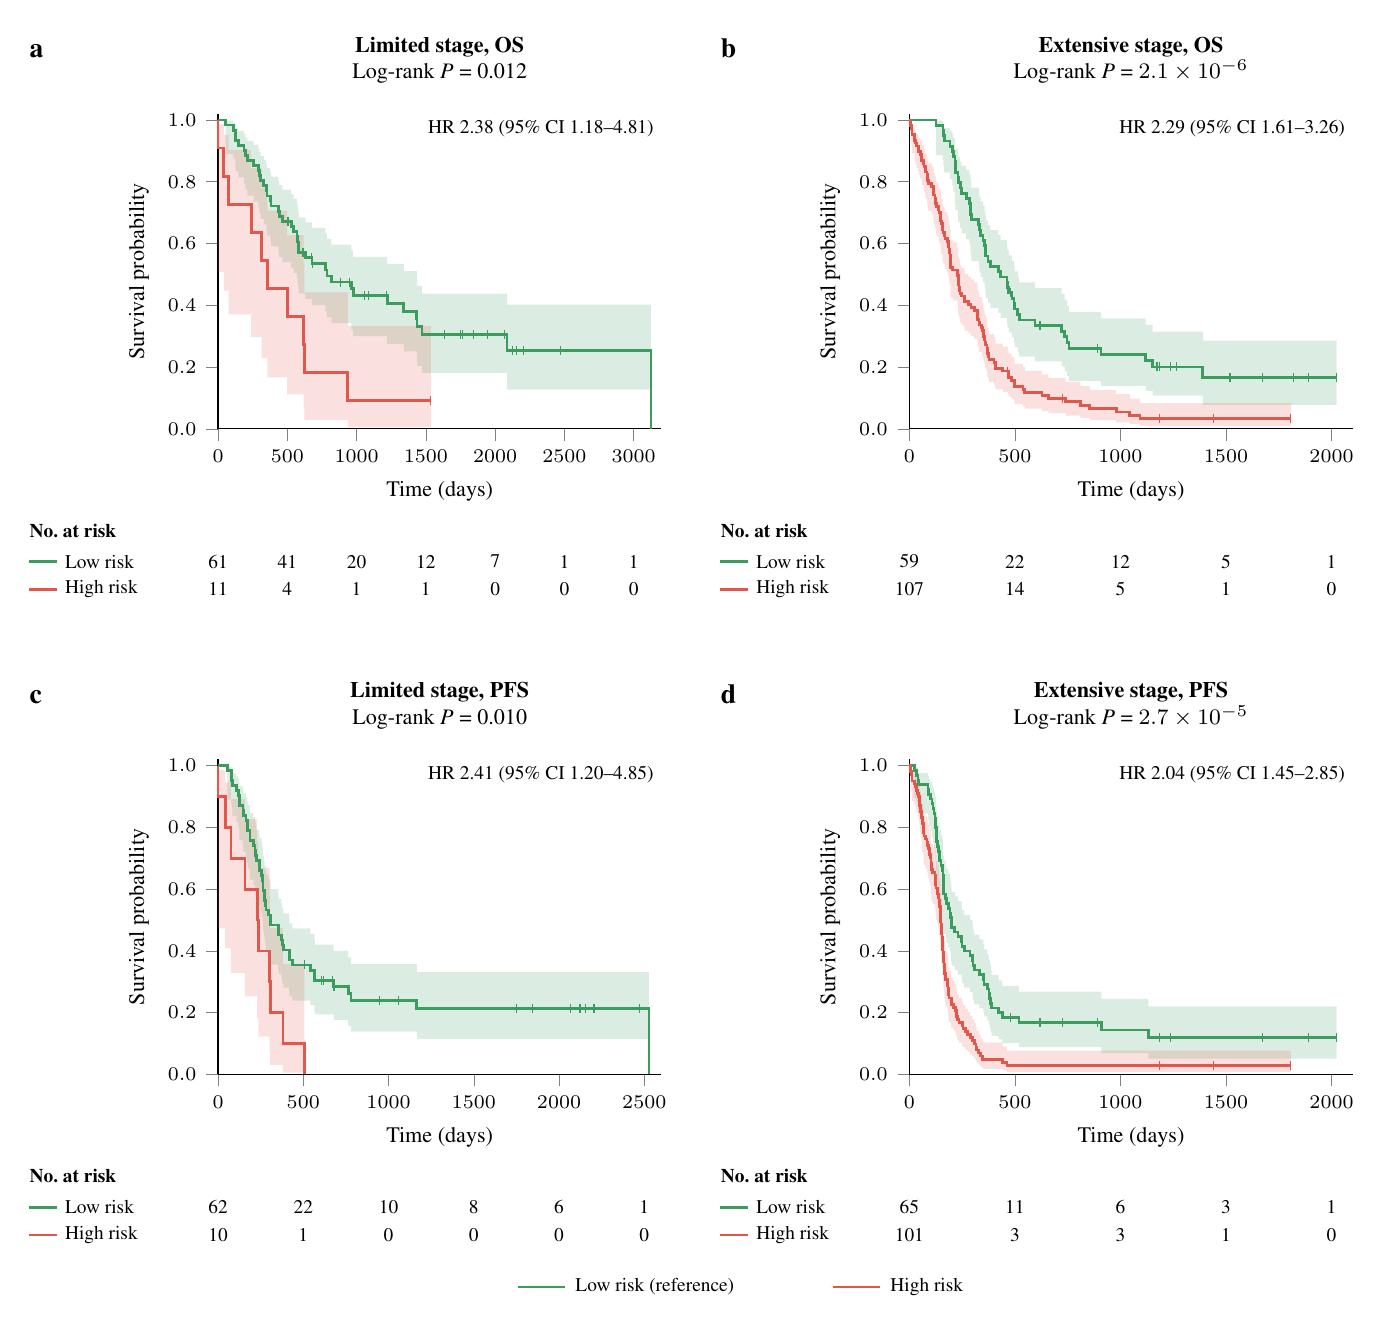
\begin{tikzpicture}
\begin{groupplot}[kmaxis, group style={group size=2 by 2, horizontal sep=31.5mm, vertical sep=42mm}]
\nextgroupplot[xmax=3200, xtick={0,500,1000,1500,2000,2500,3000}, title={\textbf{Limited stage, OS}\\ Log-rank \textit{P} = 0.012}]
\addplot[draw=none, fill=kmlow, fill opacity=0.18, forget plot] coordinates {(0.0,1.0000) (55.0,1.0000) (55.0,0.9977) (110.0,0.9977) (110.0,0.9917) (125.0,0.9917) (125.0,0.9749) (146.0,0.9749) (146.0,0.9650) (187.0,0.9650) (187.0,0.9546) (197.0,0.9546) (197.0,0.9436) (211.0,0.9436) (211.0,0.9321) (257.0,0.9321) (257.0,0.9204) (292.0,0.9204) (292.0,0.9082) (299.0,0.9082) (299.0,0.8958) (307.0,0.8958) (307.0,0.8831) (330.0,0.8831) (330.0,0.8702) (349.0,0.8702) (349.0,0.8571) (353.0,0.8571) (353.0,0.8438) (377.0,0.8438) (377.0,0.8303) (383.0,0.8303) (383.0,0.8166) (436.0,0.8166) (436.0,0.8027) (441.0,0.8027) (441.0,0.7887) (465.0,0.7887) (465.0,0.7745) (505.0,0.7745) (505.0,0.7745) (528.0,0.7745) (528.0,0.7598) (546.0,0.7598) (546.0,0.7451) (570.0,0.7451) (570.0,0.7302) (575.0,0.7302) (575.0,0.7151) (580.0,0.7151) (580.0,0.6999) (583.0,0.6999) (583.0,0.6845) (609.0,0.6845) (609.0,0.6845) (620.0,0.6845) (620.0,0.6845) (630.0,0.6845) (630.0,0.6683) (672.0,0.6683) (672.0,0.6683) (674.0,0.6683) (674.0,0.6683) (678.0,0.6683) (678.0,0.6510) (680.0,0.6510) (680.0,0.6510) (774.0,0.6510) (774.0,0.6331) (786.0,0.6331) (786.0,0.6150) (818.0,0.6150) (818.0,0.5966) (882.0,0.5966) (882.0,0.5966) (949.0,0.5966) (949.0,0.5966) (962.0,0.5966) (962.0,0.5768) (976.0,0.5768) (976.0,0.5567) (1060.0,0.5567) (1060.0,0.5567) (1086.0,0.5567) (1086.0,0.5567) (1214.0,0.5567) (1214.0,0.5567) (1221.0,0.5567) (1221.0,0.5339) (1341.0,0.5339) (1341.0,0.5106) (1435.0,0.5106) (1435.0,0.4867) (1437.0,0.4867) (1437.0,0.4624) (1472.0,0.4624) (1472.0,0.4375) (1633.0,0.4375) (1633.0,0.4375) (1750.0,0.4375) (1750.0,0.4375) (1767.0,0.4375) (1767.0,0.4375) (1843.0,0.4375) (1843.0,0.4375) (1948.0,0.4375) (1948.0,0.4375) (2066.0,0.4375) (2066.0,0.4375) (2086.0,0.4375) (2086.0,0.4023) (2123.0,0.4023) (2123.0,0.4023) (2156.0,0.4023) (2156.0,0.4023) (2205.0,0.4023) (2205.0,0.4023) (2473.0,0.4023) (2473.0,0.4023) (3125.0,0.4023) (3125.0,0.0000) (3125.0,0.0000) (3125.0,0.0000) (3125.0,0.0000) (3125.0,0.1272) (2473.0,0.1272) (2473.0,0.1272) (2205.0,0.1272) (2205.0,0.1272) (2156.0,0.1272) (2156.0,0.1272) (2123.0,0.1272) (2123.0,0.1272) (2086.0,0.1272) (2086.0,0.1813) (2066.0,0.1813) (2066.0,0.1813) (1948.0,0.1813) (1948.0,0.1813) (1843.0,0.1813) (1843.0,0.1813) (1767.0,0.1813) (1767.0,0.1813) (1750.0,0.1813) (1750.0,0.1813) (1633.0,0.1813) (1633.0,0.1813) (1472.0,0.1813) (1472.0,0.2036) (1437.0,0.2036) (1437.0,0.2266) (1435.0,0.2266) (1435.0,0.2503) (1341.0,0.2503) (1341.0,0.2748) (1221.0,0.2748) (1221.0,0.3000) (1214.0,0.3000) (1214.0,0.3000) (1086.0,0.3000) (1086.0,0.3000) (1060.0,0.3000) (1060.0,0.3000) (976.0,0.3000) (976.0,0.3208) (962.0,0.3208) (962.0,0.3420) (949.0,0.3420) (949.0,0.3420) (882.0,0.3420) (882.0,0.3420) (818.0,0.3420) (818.0,0.3612) (786.0,0.3612) (786.0,0.3807) (774.0,0.3807) (774.0,0.4005) (680.0,0.4005) (680.0,0.4005) (678.0,0.4005) (678.0,0.4197) (674.0,0.4197) (674.0,0.4197) (672.0,0.4197) (672.0,0.4197) (630.0,0.4197) (630.0,0.4374) (620.0,0.4374) (620.0,0.4374) (609.0,0.4374) (609.0,0.4374) (583.0,0.4374) (583.0,0.4540) (580.0,0.4540) (580.0,0.4707) (575.0,0.4707) (575.0,0.4876) (570.0,0.4876) (570.0,0.5047) (546.0,0.5047) (546.0,0.5219) (528.0,0.5219) (528.0,0.5392) (505.0,0.5392) (505.0,0.5392) (465.0,0.5392) (465.0,0.5562) (441.0,0.5562) (441.0,0.5733) (436.0,0.5733) (436.0,0.5906) (383.0,0.5906) (383.0,0.6080) (377.0,0.6080) (377.0,0.6257) (353.0,0.6257) (353.0,0.6435) (349.0,0.6435) (349.0,0.6615) (330.0,0.6615) (330.0,0.6797) (307.0,0.6797) (307.0,0.6981) (299.0,0.6981) (299.0,0.7167) (292.0,0.7167) (292.0,0.7356) (257.0,0.7356) (257.0,0.7548) (211.0,0.7548) (211.0,0.7743) (197.0,0.7743) (197.0,0.7941) (187.0,0.7941) (187.0,0.8142) (146.0,0.8142) (146.0,0.8347) (125.0,0.8347) (125.0,0.8752) (110.0,0.8752) (110.0,0.8893) (55.0,0.8893) (55.0,1.0000) (0.0,1.0000)} -- cycle;
\addplot[draw=none, fill=kmhigh, fill opacity=0.18, forget plot] coordinates {(0.0,0.9867) (42.0,0.9867) (42.0,0.9512) (76.0,0.9512) (76.0,0.9028) (239.0,0.9028) (239.0,0.8452) (315.0,0.8452) (315.0,0.7796) (357.0,0.7796) (357.0,0.7069) (499.0,0.7069) (499.0,0.6268) (618.0,0.6268) (618.0,0.5389) (623.0,0.5389) (623.0,0.4417) (937.0,0.4417) (937.0,0.3329) (1536.0,0.3329) (1536.0,0.3329) (1536.0,0.3329) (1536.0,0.0054) (1536.0,0.0054) (1536.0,0.0054) (937.0,0.0054) (937.0,0.0285) (623.0,0.0285) (623.0,0.0652) (618.0,0.0652) (618.0,0.1118) (499.0,0.1118) (499.0,0.1666) (357.0,0.1666) (357.0,0.2285) (315.0,0.2285) (315.0,0.2969) (239.0,0.2969) (239.0,0.3708) (76.0,0.3708) (76.0,0.4474) (42.0,0.4474) (42.0,0.5081) (0.0,0.5081)} -- cycle;
\addplot[const plot, kmlowline, forget plot] coordinates {(0.0,1.0000) (0.0,1.0000) (55.0,0.9836) (110.0,0.9672) (125.0,0.9344) (146.0,0.9180) (187.0,0.9016) (197.0,0.8852) (211.0,0.8689) (257.0,0.8525) (292.0,0.8361) (299.0,0.8197) (307.0,0.8033) (330.0,0.7869) (349.0,0.7705) (353.0,0.7541) (377.0,0.7377) (383.0,0.7213) (436.0,0.7049) (441.0,0.6885) (465.0,0.6721) (505.0,0.6721) (528.0,0.6553) (546.0,0.6385) (570.0,0.6217) (575.0,0.6049) (580.0,0.5881) (583.0,0.5713) (609.0,0.5713) (620.0,0.5713) (630.0,0.5535) (672.0,0.5535) (674.0,0.5535) (678.0,0.5344) (680.0,0.5344) (774.0,0.5146) (786.0,0.4948) (818.0,0.4750) (882.0,0.4750) (949.0,0.4750) (962.0,0.4534) (976.0,0.4318) (1060.0,0.4318) (1086.0,0.4318) (1214.0,0.4318) (1221.0,0.4064) (1341.0,0.3810) (1435.0,0.3556) (1437.0,0.3302) (1472.0,0.3048) (1633.0,0.3048) (1750.0,0.3048) (1767.0,0.3048) (1843.0,0.3048) (1948.0,0.3048) (2066.0,0.3048) (2086.0,0.2540) (2123.0,0.2540) (2156.0,0.2540) (2205.0,0.2540) (2473.0,0.2540) (3125.0,0.0000) (3125.0,0.0000)};
\addplot[only marks, mark=|, mark size=1.6pt, kmlow, forget plot] coordinates {(882.0,0.4750) (672.0,0.5535) (680.0,0.5344) (1750.0,0.3048) (2123.0,0.2540) (1060.0,0.4318) (1214.0,0.4318) (1086.0,0.4318) (2473.0,0.2540) (505.0,0.6721) (1633.0,0.3048) (2156.0,0.2540) (1843.0,0.3048) (949.0,0.4750) (2066.0,0.3048) (674.0,0.5535) (1767.0,0.3048) (2205.0,0.2540) (1948.0,0.3048) (609.0,0.5713) (620.0,0.5713)};
\addplot[const plot, kmhighline, forget plot] coordinates {(0.0,1.0000) (0.0,0.9091) (42.0,0.8182) (76.0,0.7273) (239.0,0.6364) (315.0,0.5455) (357.0,0.4545) (499.0,0.3636) (618.0,0.2727) (623.0,0.1818) (937.0,0.0909) (1536.0,0.0909) (1536.0,0.0909)};
\addplot[only marks, mark=|, mark size=1.6pt, kmhigh, forget plot] coordinates {(1536.0,0.0909)};
\node[anchor=north east, font=\kmsmall, inner sep=1pt] at (rel axis cs:0.99,0.99) {HR 2.38 (95\% CI 1.18--4.81)};
\node[anchor=south west, inner sep=0pt, font=\kmletter, xshift=-24mm, yshift=7mm] at (rel axis cs:0,1) {a};
\node[anchor=west, inner sep=0pt, font=\kmsmall\bfseries, xshift=-24mm] at (axis cs:0,-0.33) {No.\ at risk};
\draw[kmlowline] ([xshift=-24mm]axis cs:0,-0.43) -- ([xshift=-20.5mm]axis cs:0,-0.43);
\node[anchor=west, inner sep=0pt, font=\kmsmall, xshift=-19.5mm] at (axis cs:0,-0.43) {Low risk};
\node[font=\kmsmall] at (axis cs:0,-0.43) {61};
\node[font=\kmsmall] at (axis cs:500,-0.43) {41};
\node[font=\kmsmall] at (axis cs:1000,-0.43) {20};
\node[font=\kmsmall] at (axis cs:1500,-0.43) {12};
\node[font=\kmsmall] at (axis cs:2000,-0.43) {7};
\node[font=\kmsmall] at (axis cs:2500,-0.43) {1};
\node[font=\kmsmall] at (axis cs:3000,-0.43) {1};
\draw[kmhighline] ([xshift=-24mm]axis cs:0,-0.52) -- ([xshift=-20.5mm]axis cs:0,-0.52);
\node[anchor=west, inner sep=0pt, font=\kmsmall, xshift=-19.5mm] at (axis cs:0,-0.52) {High risk};
\node[font=\kmsmall] at (axis cs:0,-0.52) {11};
\node[font=\kmsmall] at (axis cs:500,-0.52) {4};
\node[font=\kmsmall] at (axis cs:1000,-0.52) {1};
\node[font=\kmsmall] at (axis cs:1500,-0.52) {1};
\node[font=\kmsmall] at (axis cs:2000,-0.52) {0};
\node[font=\kmsmall] at (axis cs:2500,-0.52) {0};
\node[font=\kmsmall] at (axis cs:3000,-0.52) {0};
\nextgroupplot[xmax=2100, xtick={0,500,1000,1500,2000}, title={\textbf{Extensive stage, OS}\\ Log-rank \textit{P} = $2.1\times10^{-6}$}]
\addplot[draw=none, fill=kmlow, fill opacity=0.18, forget plot] coordinates {(0.0,1.0000) (126.0,1.0000) (126.0,0.9976) (159.0,0.9976) (159.0,0.9914) (161.0,0.9914) (161.0,0.9833) (165.0,0.9833) (165.0,0.9740) (193.0,0.9740) (193.0,0.9638) (204.0,0.9638) (204.0,0.9530) (209.0,0.9530) (209.0,0.9416) (216.0,0.9416) (216.0,0.9298) (217.0,0.9298) (217.0,0.9175) (218.0,0.9175) (218.0,0.9050) (230.0,0.9050) (230.0,0.8921) (231.0,0.8921) (231.0,0.8790) (241.0,0.8790) (241.0,0.8656) (247.0,0.8656) (247.0,0.8520) (269.0,0.8520) (269.0,0.8382) (284.0,0.8382) (284.0,0.8242) (289.0,0.8242) (289.0,0.8099) (291.0,0.8099) (291.0,0.7955) (294.0,0.7955) (294.0,0.7810) (329.0,0.7810) (329.0,0.7663) (332.0,0.7663) (332.0,0.7514) (338.0,0.7514) (338.0,0.7363) (349.0,0.7363) (349.0,0.7211) (356.0,0.7211) (356.0,0.7058) (360.0,0.7058) (360.0,0.6903) (362.0,0.6903) (362.0,0.6747) (373.0,0.6747) (373.0,0.6590) (384.0,0.6590) (384.0,0.6431) (422.0,0.6431) (422.0,0.6270) (432.0,0.6270) (432.0,0.6109) (462.0,0.6109) (462.0,0.5946) (464.0,0.5946) (464.0,0.5782) (471.0,0.5782) (471.0,0.5616) (478.0,0.5616) (478.0,0.5616) (486.0,0.5616) (486.0,0.5444) (496.0,0.5444) (496.0,0.5270) (499.0,0.5270) (499.0,0.5095) (514.0,0.5095) (514.0,0.4918) (520.0,0.4918) (520.0,0.4739) (595.0,0.4739) (595.0,0.4559) (619.0,0.4559) (619.0,0.4559) (721.0,0.4559) (721.0,0.4369) (735.0,0.4369) (735.0,0.4177) (747.0,0.4177) (747.0,0.3983) (756.0,0.3983) (756.0,0.3787) (893.0,0.3787) (893.0,0.3787) (908.0,0.3787) (908.0,0.3577) (1119.0,0.3577) (1119.0,0.3364) (1152.0,0.3364) (1152.0,0.3147) (1173.0,0.3147) (1173.0,0.3147) (1184.0,0.3147) (1184.0,0.3147) (1239.0,0.3147) (1239.0,0.3147) (1267.0,0.3147) (1267.0,0.3147) (1390.0,0.3147) (1390.0,0.2859) (1519.0,0.2859) (1519.0,0.2859) (1673.0,0.2859) (1673.0,0.2859) (1821.0,0.2859) (1821.0,0.2859) (1890.0,0.2859) (1890.0,0.2859) (2024.0,0.2859) (2024.0,0.2859) (2024.0,0.2859) (2024.0,0.0774) (2024.0,0.0774) (2024.0,0.0774) (1890.0,0.0774) (1890.0,0.0774) (1821.0,0.0774) (1821.0,0.0774) (1673.0,0.0774) (1673.0,0.0774) (1519.0,0.0774) (1519.0,0.0774) (1390.0,0.0774) (1390.0,0.1070) (1267.0,0.1070) (1267.0,0.1070) (1239.0,0.1070) (1239.0,0.1070) (1184.0,0.1070) (1184.0,0.1070) (1173.0,0.1070) (1173.0,0.1070) (1152.0,0.1070) (1152.0,0.1226) (1119.0,0.1226) (1119.0,0.1386) (908.0,0.1386) (908.0,0.1551) (893.0,0.1551) (893.0,0.1551) (756.0,0.1551) (756.0,0.1704) (747.0,0.1704) (747.0,0.1860) (735.0,0.1860) (735.0,0.2019) (721.0,0.2019) (721.0,0.2180) (619.0,0.2180) (619.0,0.2180) (595.0,0.2180) (595.0,0.2333) (520.0,0.2333) (520.0,0.2487) (514.0,0.2487) (514.0,0.2643) (499.0,0.2643) (499.0,0.2801) (496.0,0.2801) (496.0,0.2961) (486.0,0.2961) (486.0,0.3123) (478.0,0.3123) (478.0,0.3123) (471.0,0.3123) (471.0,0.3278) (464.0,0.3278) (464.0,0.3435) (462.0,0.3435) (462.0,0.3593) (432.0,0.3593) (432.0,0.3753) (422.0,0.3753) (422.0,0.3914) (384.0,0.3914) (384.0,0.4076) (373.0,0.4076) (373.0,0.4240) (362.0,0.4240) (362.0,0.4405) (360.0,0.4405) (360.0,0.4572) (356.0,0.4572) (356.0,0.4740) (349.0,0.4740) (349.0,0.4910) (338.0,0.4910) (338.0,0.5081) (332.0,0.5081) (332.0,0.5254) (329.0,0.5254) (329.0,0.5428) (294.0,0.5428) (294.0,0.5604) (291.0,0.5604) (291.0,0.5781) (289.0,0.5781) (289.0,0.5961) (284.0,0.5961) (284.0,0.6142) (269.0,0.6142) (269.0,0.6325) (247.0,0.6325) (247.0,0.6510) (241.0,0.6510) (241.0,0.6697) (231.0,0.6697) (231.0,0.6887) (230.0,0.6887) (230.0,0.7079) (218.0,0.7079) (218.0,0.7274) (217.0,0.7274) (217.0,0.7471) (216.0,0.7471) (216.0,0.7672) (209.0,0.7672) (209.0,0.7876) (204.0,0.7876) (204.0,0.8083) (193.0,0.8083) (193.0,0.8294) (165.0,0.8294) (165.0,0.8506) (161.0,0.8506) (161.0,0.8712) (159.0,0.8712) (159.0,0.8857) (126.0,0.8857) (126.0,1.0000) (0.0,1.0000)} -- cycle;
\addplot[draw=none, fill=kmhigh, fill opacity=0.18, forget plot] coordinates {(0.0,1.0000) (6.0,1.0000) (6.0,0.9953) (10.0,0.9953) (10.0,0.9909) (12.0,0.9909) (12.0,0.9803) (24.0,0.9803) (24.0,0.9683) (30.0,0.9683) (30.0,0.9619) (33.0,0.9619) (33.0,0.9553) (42.0,0.9553) (42.0,0.9486) (45.0,0.9486) (45.0,0.9417) (51.0,0.9417) (51.0,0.9347) (58.0,0.9347) (58.0,0.9276) (59.0,0.9276) (59.0,0.9203) (67.0,0.9203) (67.0,0.9130) (69.0,0.9130) (69.0,0.9056) (76.0,0.9056) (76.0,0.8905) (84.0,0.8905) (84.0,0.8828) (85.0,0.8828) (85.0,0.8751) (87.0,0.8751) (87.0,0.8673) (90.0,0.8673) (90.0,0.8595) (106.0,0.8595) (106.0,0.8516) (114.0,0.8516) (114.0,0.8436) (115.0,0.8436) (115.0,0.8356) (116.0,0.8356) (116.0,0.8275) (121.0,0.8275) (121.0,0.8194) (124.0,0.8194) (124.0,0.8113) (125.0,0.8113) (125.0,0.8030) (128.0,0.8030) (128.0,0.7948) (139.0,0.7948) (139.0,0.7865) (140.0,0.7865) (140.0,0.7782) (147.0,0.7782) (147.0,0.7698) (149.0,0.7698) (149.0,0.7529) (151.0,0.7529) (151.0,0.7444) (157.0,0.7444) (157.0,0.7359) (158.0,0.7359) (158.0,0.7273) (159.0,0.7273) (159.0,0.7187) (167.0,0.7187) (167.0,0.7101) (169.0,0.7101) (169.0,0.7014) (179.0,0.7014) (179.0,0.6927) (184.0,0.6927) (184.0,0.6839) (186.0,0.6839) (186.0,0.6751) (188.0,0.6751) (188.0,0.6663) (189.0,0.6663) (189.0,0.6575) (193.0,0.6575) (193.0,0.6486) (195.0,0.6486) (195.0,0.6218) (196.0,0.6218) (196.0,0.6128) (206.0,0.6128) (206.0,0.6038) (227.0,0.6038) (227.0,0.5856) (231.0,0.5856) (231.0,0.5673) (232.0,0.5673) (232.0,0.5581) (235.0,0.5581) (235.0,0.5489) (239.0,0.5489) (239.0,0.5397) (240.0,0.5397) (240.0,0.5304) (247.0,0.5304) (247.0,0.5210) (261.0,0.5210) (261.0,0.5117) (262.0,0.5117) (262.0,0.5023) (279.0,0.5023) (279.0,0.4929) (292.0,0.4929) (292.0,0.4835) (307.0,0.4835) (307.0,0.4740) (322.0,0.4740) (322.0,0.4645) (323.0,0.4645) (323.0,0.4453) (330.0,0.4453) (330.0,0.4357) (331.0,0.4357) (331.0,0.4260) (343.0,0.4260) (343.0,0.4163) (346.0,0.4163) (346.0,0.4066) (351.0,0.4066) (351.0,0.3968) (352.0,0.3968) (352.0,0.3870) (357.0,0.3870) (357.0,0.3772) (358.0,0.3772) (358.0,0.3673) (362.0,0.3673) (362.0,0.3574) (368.0,0.3574) (368.0,0.3474) (370.0,0.3474) (370.0,0.3273) (375.0,0.3273) (375.0,0.3172) (377.0,0.3172) (377.0,0.3070) (401.0,0.3070) (401.0,0.2968) (408.0,0.2968) (408.0,0.2865) (409.0,0.2865) (409.0,0.2762) (443.0,0.2762) (443.0,0.2658) (465.0,0.2658) (465.0,0.2658) (468.0,0.2658) (468.0,0.2549) (470.0,0.2549) (470.0,0.2440) (484.0,0.2440) (484.0,0.2329) (498.0,0.2329) (498.0,0.2218) (499.0,0.2218) (499.0,0.2106) (538.0,0.2106) (538.0,0.1993) (547.0,0.1993) (547.0,0.1878) (628.0,0.1878) (628.0,0.1762) (659.0,0.1762) (659.0,0.1645) (725.0,0.1645) (725.0,0.1645) (740.0,0.1645) (740.0,0.1518) (810.0,0.1518) (810.0,0.1389) (855.0,0.1389) (855.0,0.1256) (980.0,0.1256) (980.0,0.1120) (1044.0,0.1120) (1044.0,0.0980) (1092.0,0.0980) (1092.0,0.0835) (1184.0,0.0835) (1184.0,0.0835) (1439.0,0.0835) (1439.0,0.0835) (1807.0,0.0835) (1807.0,0.0835) (1807.0,0.0835) (1807.0,0.0091) (1807.0,0.0091) (1807.0,0.0091) (1439.0,0.0091) (1439.0,0.0091) (1184.0,0.0091) (1184.0,0.0091) (1092.0,0.0091) (1092.0,0.0147) (1044.0,0.0147) (1044.0,0.0211) (980.0,0.0211) (980.0,0.0279) (855.0,0.0279) (855.0,0.0352) (810.0,0.0352) (810.0,0.0428) (740.0,0.0428) (740.0,0.0508) (725.0,0.0508) (725.0,0.0508) (659.0,0.0508) (659.0,0.0579) (628.0,0.0579) (628.0,0.0652) (547.0,0.0652) (547.0,0.0727) (538.0,0.0727) (538.0,0.0802) (499.0,0.0802) (499.0,0.0879) (498.0,0.0879) (498.0,0.0957) (484.0,0.0957) (484.0,0.1036) (470.0,0.1036) (470.0,0.1116) (468.0,0.1116) (468.0,0.1197) (465.0,0.1197) (465.0,0.1197) (443.0,0.1197) (443.0,0.1274) (409.0,0.1274) (409.0,0.1351) (408.0,0.1351) (408.0,0.1429) (401.0,0.1429) (401.0,0.1507) (377.0,0.1507) (377.0,0.1587) (375.0,0.1587) (375.0,0.1666) (370.0,0.1666) (370.0,0.1827) (368.0,0.1827) (368.0,0.1908) (362.0,0.1908) (362.0,0.1990) (358.0,0.1990) (358.0,0.2072) (357.0,0.2072) (357.0,0.2155) (352.0,0.2155) (352.0,0.2238) (351.0,0.2238) (351.0,0.2321) (346.0,0.2321) (346.0,0.2405) (343.0,0.2405) (343.0,0.2489) (331.0,0.2489) (331.0,0.2574) (330.0,0.2574) (330.0,0.2659) (323.0,0.2659) (323.0,0.2830) (322.0,0.2830) (322.0,0.2916) (307.0,0.2916) (307.0,0.3002) (292.0,0.3002) (292.0,0.3089) (279.0,0.3089) (279.0,0.3176) (262.0,0.3176) (262.0,0.3264) (261.0,0.3264) (261.0,0.3352) (247.0,0.3352) (247.0,0.3440) (240.0,0.3440) (240.0,0.3528) (239.0,0.3528) (239.0,0.3617) (235.0,0.3617) (235.0,0.3706) (232.0,0.3706) (232.0,0.3796) (231.0,0.3796) (231.0,0.3976) (227.0,0.3976) (227.0,0.4157) (206.0,0.4157) (206.0,0.4248) (196.0,0.4248) (196.0,0.4340) (195.0,0.4340) (195.0,0.4616) (193.0,0.4616) (193.0,0.4709) (189.0,0.4709) (189.0,0.4802) (188.0,0.4802) (188.0,0.4896) (186.0,0.4896) (186.0,0.4989) (184.0,0.4989) (184.0,0.5084) (179.0,0.5084) (179.0,0.5178) (169.0,0.5178) (169.0,0.5273) (167.0,0.5273) (167.0,0.5368) (159.0,0.5368) (159.0,0.5464) (158.0,0.5464) (158.0,0.5559) (157.0,0.5559) (157.0,0.5656) (151.0,0.5656) (151.0,0.5752) (149.0,0.5752) (149.0,0.5947) (147.0,0.5947) (147.0,0.6045) (140.0,0.6045) (140.0,0.6143) (139.0,0.6143) (139.0,0.6242) (128.0,0.6242) (128.0,0.6341) (125.0,0.6341) (125.0,0.6440) (124.0,0.6440) (124.0,0.6540) (121.0,0.6540) (121.0,0.6641) (116.0,0.6641) (116.0,0.6742) (115.0,0.6742) (115.0,0.6843) (114.0,0.6843) (114.0,0.6945) (106.0,0.6945) (106.0,0.7048) (90.0,0.7048) (90.0,0.7151) (87.0,0.7151) (87.0,0.7254) (85.0,0.7254) (85.0,0.7359) (84.0,0.7359) (84.0,0.7464) (76.0,0.7464) (76.0,0.7676) (69.0,0.7676) (69.0,0.7783) (67.0,0.7783) (67.0,0.7891) (59.0,0.7891) (59.0,0.8000) (58.0,0.8000) (58.0,0.8110) (51.0,0.8110) (51.0,0.8221) (45.0,0.8221) (45.0,0.8333) (42.0,0.8333) (42.0,0.8446) (33.0,0.8446) (33.0,0.8561) (30.0,0.8561) (30.0,0.8677) (24.0,0.8677) (24.0,0.8914) (12.0,0.8914) (12.0,0.9156) (10.0,0.9156) (10.0,0.9273) (6.0,0.9273) (6.0,1.0000) (0.0,1.0000)} -- cycle;
\addplot[const plot, kmlowline, forget plot] coordinates {(0.0,1.0000) (0.0,1.0000) (126.0,0.9831) (159.0,0.9661) (161.0,0.9492) (165.0,0.9322) (193.0,0.9153) (204.0,0.8983) (209.0,0.8814) (216.0,0.8644) (217.0,0.8475) (218.0,0.8305) (230.0,0.8136) (231.0,0.7966) (241.0,0.7797) (247.0,0.7627) (269.0,0.7458) (284.0,0.7288) (289.0,0.7119) (291.0,0.6949) (294.0,0.6780) (329.0,0.6610) (332.0,0.6441) (338.0,0.6271) (349.0,0.6102) (356.0,0.5932) (360.0,0.5763) (362.0,0.5593) (373.0,0.5424) (384.0,0.5254) (422.0,0.5085) (432.0,0.4915) (462.0,0.4746) (464.0,0.4576) (471.0,0.4407) (478.0,0.4407) (486.0,0.4231) (496.0,0.4054) (499.0,0.3878) (514.0,0.3702) (520.0,0.3525) (595.0,0.3349) (619.0,0.3349) (721.0,0.3163) (735.0,0.2977) (747.0,0.2791) (756.0,0.2605) (893.0,0.2605) (908.0,0.2405) (1119.0,0.2204) (1152.0,0.2004) (1173.0,0.2004) (1184.0,0.2004) (1239.0,0.2004) (1267.0,0.2004) (1390.0,0.1670) (1519.0,0.1670) (1673.0,0.1670) (1821.0,0.1670) (1890.0,0.1670) (2024.0,0.1670) (2024.0,0.1670)};
\addplot[only marks, mark=|, mark size=1.6pt, kmlow, forget plot] coordinates {(893.0,0.2605) (1890.0,0.1670) (1673.0,0.1670) (1267.0,0.2004) (1821.0,0.1670) (1239.0,0.2004) (1173.0,0.2004) (478.0,0.4407) (2024.0,0.1670) (1519.0,0.1670) (619.0,0.3349) (1184.0,0.2004)};
\addplot[const plot, kmhighline, forget plot] coordinates {(0.0,1.0000) (0.0,1.0000) (6.0,0.9813) (10.0,0.9720) (12.0,0.9533) (24.0,0.9346) (30.0,0.9252) (33.0,0.9159) (42.0,0.9065) (45.0,0.8972) (51.0,0.8879) (58.0,0.8785) (59.0,0.8692) (67.0,0.8598) (69.0,0.8505) (76.0,0.8318) (84.0,0.8224) (85.0,0.8131) (87.0,0.8037) (90.0,0.7944) (106.0,0.7850) (114.0,0.7757) (115.0,0.7664) (116.0,0.7570) (121.0,0.7477) (124.0,0.7383) (125.0,0.7290) (128.0,0.7196) (139.0,0.7103) (140.0,0.7009) (147.0,0.6916) (149.0,0.6729) (151.0,0.6636) (157.0,0.6542) (158.0,0.6449) (159.0,0.6355) (167.0,0.6262) (169.0,0.6168) (179.0,0.6075) (184.0,0.5981) (186.0,0.5888) (188.0,0.5794) (189.0,0.5701) (193.0,0.5607) (195.0,0.5327) (196.0,0.5234) (206.0,0.5140) (227.0,0.4953) (231.0,0.4766) (232.0,0.4673) (235.0,0.4579) (239.0,0.4486) (240.0,0.4393) (247.0,0.4299) (261.0,0.4206) (262.0,0.4112) (279.0,0.4019) (292.0,0.3925) (307.0,0.3832) (322.0,0.3738) (323.0,0.3551) (330.0,0.3458) (331.0,0.3364) (343.0,0.3271) (346.0,0.3178) (351.0,0.3084) (352.0,0.2991) (357.0,0.2897) (358.0,0.2804) (362.0,0.2710) (368.0,0.2617) (370.0,0.2430) (375.0,0.2336) (377.0,0.2243) (401.0,0.2150) (408.0,0.2056) (409.0,0.1963) (443.0,0.1869) (465.0,0.1869) (468.0,0.1771) (470.0,0.1672) (484.0,0.1574) (498.0,0.1476) (499.0,0.1377) (538.0,0.1279) (547.0,0.1181) (628.0,0.1082) (659.0,0.0984) (725.0,0.0984) (740.0,0.0874) (810.0,0.0765) (855.0,0.0656) (980.0,0.0547) (1044.0,0.0437) (1092.0,0.0328) (1184.0,0.0328) (1439.0,0.0328) (1807.0,0.0328) (1807.0,0.0328)};
\addplot[only marks, mark=|, mark size=1.6pt, kmhigh, forget plot] coordinates {(1807.0,0.0328) (1439.0,0.0328) (725.0,0.0984) (465.0,0.1869) (1184.0,0.0328)};
\node[anchor=north east, font=\kmsmall, inner sep=1pt] at (rel axis cs:0.99,0.99) {HR 2.29 (95\% CI 1.61--3.26)};
\node[anchor=south west, inner sep=0pt, font=\kmletter, xshift=-24mm, yshift=7mm] at (rel axis cs:0,1) {b};
\node[anchor=west, inner sep=0pt, font=\kmsmall\bfseries, xshift=-24mm] at (axis cs:0,-0.33) {No.\ at risk};
\draw[kmlowline] ([xshift=-24mm]axis cs:0,-0.43) -- ([xshift=-20.5mm]axis cs:0,-0.43);
\node[anchor=west, inner sep=0pt, font=\kmsmall, xshift=-19.5mm] at (axis cs:0,-0.43) {Low risk};
\node[font=\kmsmall] at (axis cs:0,-0.43) {59};
\node[font=\kmsmall] at (axis cs:500,-0.43) {22};
\node[font=\kmsmall] at (axis cs:1000,-0.43) {12};
\node[font=\kmsmall] at (axis cs:1500,-0.43) {5};
\node[font=\kmsmall] at (axis cs:2000,-0.43) {1};
\draw[kmhighline] ([xshift=-24mm]axis cs:0,-0.52) -- ([xshift=-20.5mm]axis cs:0,-0.52);
\node[anchor=west, inner sep=0pt, font=\kmsmall, xshift=-19.5mm] at (axis cs:0,-0.52) {High risk};
\node[font=\kmsmall] at (axis cs:0,-0.52) {107};
\node[font=\kmsmall] at (axis cs:500,-0.52) {14};
\node[font=\kmsmall] at (axis cs:1000,-0.52) {5};
\node[font=\kmsmall] at (axis cs:1500,-0.52) {1};
\node[font=\kmsmall] at (axis cs:2000,-0.52) {0};
\nextgroupplot[xmax=2600, xtick={0,500,1000,1500,2000,2500}, title={\textbf{Limited stage, PFS}\\ Log-rank \textit{P} = 0.010}]
\addplot[draw=none, fill=kmlow, fill opacity=0.18, forget plot] coordinates {(0.0,1.0000) (55.0,1.0000) (55.0,0.9977) (77.0,0.9977) (77.0,0.9918) (81.0,0.9918) (81.0,0.9841) (84.0,0.9841) (84.0,0.9753) (108.0,0.9753) (108.0,0.9656) (119.0,0.9656) (119.0,0.9553) (125.0,0.9553) (125.0,0.9333) (146.0,0.9333) (146.0,0.9217) (149.0,0.9217) (149.0,0.9098) (164.0,0.9098) (164.0,0.8976) (171.0,0.8976) (171.0,0.8851) (173.0,0.8851) (173.0,0.8724) (187.0,0.8724) (187.0,0.8464) (208.0,0.8464) (208.0,0.8332) (217.0,0.8332) (217.0,0.8197) (220.0,0.8197) (220.0,0.8061) (225.0,0.8061) (225.0,0.7923) (241.0,0.7923) (241.0,0.7784) (244.0,0.7784) (244.0,0.7643) (256.0,0.7643) (256.0,0.7501) (260.0,0.7501) (260.0,0.7357) (264.0,0.7357) (264.0,0.7066) (271.0,0.7066) (271.0,0.6919) (273.0,0.6919) (273.0,0.6770) (277.0,0.6770) (277.0,0.6620) (282.0,0.6620) (282.0,0.6469) (297.0,0.6469) (297.0,0.6317) (307.0,0.6317) (307.0,0.6163) (309.0,0.6163) (309.0,0.6008) (353.0,0.6008) (353.0,0.5852) (356.0,0.5852) (356.0,0.5695) (372.0,0.5695) (372.0,0.5537) (376.0,0.5537) (376.0,0.5377) (383.0,0.5377) (383.0,0.5217) (417.0,0.5217) (417.0,0.5055) (418.0,0.5055) (418.0,0.4891) (436.0,0.4891) (436.0,0.4727) (505.0,0.4727) (505.0,0.4727) (541.0,0.4727) (541.0,0.4555) (565.0,0.4555) (565.0,0.4381) (568.0,0.4381) (568.0,0.4206) (609.0,0.4206) (609.0,0.4206) (620.0,0.4206) (620.0,0.4206) (672.0,0.4206) (672.0,0.4206) (678.0,0.4206) (678.0,0.4004) (680.0,0.4004) (680.0,0.4004) (763.0,0.4004) (763.0,0.3789) (780.0,0.3789) (780.0,0.3569) (949.0,0.3569) (949.0,0.3569) (1060.0,0.3569) (1060.0,0.3569) (1166.0,0.3569) (1166.0,0.3316) (1750.0,0.3316) (1750.0,0.3316) (1843.0,0.3316) (1843.0,0.3316) (2066.0,0.3316) (2066.0,0.3316) (2123.0,0.3316) (2123.0,0.3316) (2156.0,0.3316) (2156.0,0.3316) (2205.0,0.3316) (2205.0,0.3316) (2473.0,0.3316) (2473.0,0.3316) (2527.0,0.3316) (2527.0,0.0000) (2527.0,0.0000) (2527.0,0.0000) (2527.0,0.0000) (2527.0,0.1153) (2473.0,0.1153) (2473.0,0.1153) (2205.0,0.1153) (2205.0,0.1153) (2156.0,0.1153) (2156.0,0.1153) (2123.0,0.1153) (2123.0,0.1153) (2066.0,0.1153) (2066.0,0.1153) (1843.0,0.1153) (1843.0,0.1153) (1750.0,0.1153) (1750.0,0.1153) (1166.0,0.1153) (1166.0,0.1388) (1060.0,0.1388) (1060.0,0.1388) (949.0,0.1388) (949.0,0.1388) (780.0,0.1388) (780.0,0.1575) (763.0,0.1575) (763.0,0.1768) (680.0,0.1768) (680.0,0.1768) (678.0,0.1768) (678.0,0.1948) (672.0,0.1948) (672.0,0.1948) (620.0,0.1948) (620.0,0.1948) (609.0,0.1948) (609.0,0.1948) (568.0,0.1948) (568.0,0.2093) (565.0,0.2093) (565.0,0.2239) (541.0,0.2239) (541.0,0.2387) (505.0,0.2387) (505.0,0.2387) (436.0,0.2387) (436.0,0.2528) (418.0,0.2528) (418.0,0.2671) (417.0,0.2671) (417.0,0.2815) (383.0,0.2815) (383.0,0.2960) (376.0,0.2960) (376.0,0.3107) (372.0,0.3107) (372.0,0.3255) (356.0,0.3255) (356.0,0.3404) (353.0,0.3404) (353.0,0.3554) (309.0,0.3554) (309.0,0.3706) (307.0,0.3706) (307.0,0.3859) (297.0,0.3859) (297.0,0.4013) (282.0,0.4013) (282.0,0.4169) (277.0,0.4169) (277.0,0.4325) (273.0,0.4325) (273.0,0.4483) (271.0,0.4483) (271.0,0.4643) (264.0,0.4643) (264.0,0.4965) (260.0,0.4965) (260.0,0.5128) (256.0,0.5128) (256.0,0.5293) (244.0,0.5293) (244.0,0.5459) (241.0,0.5459) (241.0,0.5626) (225.0,0.5626) (225.0,0.5795) (220.0,0.5795) (220.0,0.5966) (217.0,0.5966) (217.0,0.6138) (208.0,0.6138) (208.0,0.6312) (187.0,0.6312) (187.0,0.6665) (173.0,0.6665) (173.0,0.6844) (171.0,0.6844) (171.0,0.7026) (164.0,0.7026) (164.0,0.7210) (149.0,0.7210) (149.0,0.7396) (146.0,0.7396) (146.0,0.7585) (125.0,0.7585) (125.0,0.7972) (119.0,0.7972) (119.0,0.8170) (108.0,0.8170) (108.0,0.8372) (84.0,0.8372) (84.0,0.8574) (81.0,0.8574) (81.0,0.8771) (77.0,0.8771) (77.0,0.8910) (55.0,0.8910) (55.0,1.0000) (0.0,1.0000)} -- cycle;
\addplot[draw=none, fill=kmhigh, fill opacity=0.18, forget plot] coordinates {(0.0,0.9853) (42.0,0.9853) (42.0,0.9459) (76.0,0.9459) (76.0,0.8919) (158.0,0.8919) (158.0,0.8272) (230.0,0.8272) (230.0,0.7532) (237.0,0.7532) (237.0,0.6702) (303.0,0.6702) (303.0,0.5779) (306.0,0.5779) (306.0,0.4747) (381.0,0.4747) (381.0,0.3581) (507.0,0.3581) (507.0,0.0000) (507.0,0.0000) (507.0,0.0000) (507.0,0.0000) (507.0,0.0057) (381.0,0.0057) (381.0,0.0309) (306.0,0.0309) (306.0,0.0711) (303.0,0.0711) (303.0,0.1227) (237.0,0.1227) (237.0,0.1836) (230.0,0.1836) (230.0,0.2527) (158.0,0.2527) (158.0,0.3287) (76.0,0.3287) (76.0,0.4087) (42.0,0.4087) (42.0,0.4730) (0.0,0.4730)} -- cycle;
\addplot[const plot, kmlowline, forget plot] coordinates {(0.0,1.0000) (0.0,1.0000) (55.0,0.9839) (77.0,0.9677) (81.0,0.9516) (84.0,0.9355) (108.0,0.9194) (119.0,0.9032) (125.0,0.8710) (146.0,0.8548) (149.0,0.8387) (164.0,0.8226) (171.0,0.8065) (173.0,0.7903) (187.0,0.7581) (208.0,0.7419) (217.0,0.7258) (220.0,0.7097) (225.0,0.6935) (241.0,0.6774) (244.0,0.6613) (256.0,0.6452) (260.0,0.6290) (264.0,0.5968) (271.0,0.5806) (273.0,0.5645) (277.0,0.5484) (282.0,0.5323) (297.0,0.5161) (307.0,0.5000) (309.0,0.4839) (353.0,0.4677) (356.0,0.4516) (372.0,0.4355) (376.0,0.4194) (383.0,0.4032) (417.0,0.3871) (418.0,0.3710) (436.0,0.3548) (505.0,0.3548) (541.0,0.3379) (565.0,0.3210) (568.0,0.3041) (609.0,0.3041) (620.0,0.3041) (672.0,0.3041) (678.0,0.2839) (680.0,0.2839) (763.0,0.2620) (780.0,0.2402) (949.0,0.2402) (1060.0,0.2402) (1166.0,0.2135) (1750.0,0.2135) (1843.0,0.2135) (2066.0,0.2135) (2123.0,0.2135) (2156.0,0.2135) (2205.0,0.2135) (2473.0,0.2135) (2527.0,0.0000) (2527.0,0.0000)};
\addplot[only marks, mark=|, mark size=1.6pt, kmlow, forget plot] coordinates {(672.0,0.3041) (680.0,0.2839) (1750.0,0.2135) (2123.0,0.2135) (1060.0,0.2402) (2473.0,0.2135) (505.0,0.3548) (2156.0,0.2135) (1843.0,0.2135) (949.0,0.2402) (2066.0,0.2135) (2205.0,0.2135) (609.0,0.3041) (620.0,0.3041)};
\addplot[const plot, kmhighline, forget plot] coordinates {(0.0,1.0000) (0.0,0.9000) (42.0,0.8000) (76.0,0.7000) (158.0,0.6000) (230.0,0.5000) (237.0,0.4000) (303.0,0.3000) (306.0,0.2000) (381.0,0.1000) (507.0,0.0000) (507.0,0.0000)};
\node[anchor=north east, font=\kmsmall, inner sep=1pt] at (rel axis cs:0.99,0.99) {HR 2.41 (95\% CI 1.20--4.85)};
\node[anchor=south west, inner sep=0pt, font=\kmletter, xshift=-24mm, yshift=7mm] at (rel axis cs:0,1) {c};
\node[anchor=west, inner sep=0pt, font=\kmsmall\bfseries, xshift=-24mm] at (axis cs:0,-0.33) {No.\ at risk};
\draw[kmlowline] ([xshift=-24mm]axis cs:0,-0.43) -- ([xshift=-20.5mm]axis cs:0,-0.43);
\node[anchor=west, inner sep=0pt, font=\kmsmall, xshift=-19.5mm] at (axis cs:0,-0.43) {Low risk};
\node[font=\kmsmall] at (axis cs:0,-0.43) {62};
\node[font=\kmsmall] at (axis cs:500,-0.43) {22};
\node[font=\kmsmall] at (axis cs:1000,-0.43) {10};
\node[font=\kmsmall] at (axis cs:1500,-0.43) {8};
\node[font=\kmsmall] at (axis cs:2000,-0.43) {6};
\node[font=\kmsmall] at (axis cs:2500,-0.43) {1};
\draw[kmhighline] ([xshift=-24mm]axis cs:0,-0.52) -- ([xshift=-20.5mm]axis cs:0,-0.52);
\node[anchor=west, inner sep=0pt, font=\kmsmall, xshift=-19.5mm] at (axis cs:0,-0.52) {High risk};
\node[font=\kmsmall] at (axis cs:0,-0.52) {10};
\node[font=\kmsmall] at (axis cs:500,-0.52) {1};
\node[font=\kmsmall] at (axis cs:1000,-0.52) {0};
\node[font=\kmsmall] at (axis cs:1500,-0.52) {0};
\node[font=\kmsmall] at (axis cs:2000,-0.52) {0};
\node[font=\kmsmall] at (axis cs:2500,-0.52) {0};
\nextgroupplot[xmax=2100, xtick={0,500,1000,1500,2000}, title={\textbf{Extensive stage, PFS}\\ Log-rank \textit{P} = $2.7\times10^{-5}$}]
\addplot[draw=none, fill=kmlow, fill opacity=0.18, forget plot] coordinates {(0.0,1.0000) (24.0,1.0000) (24.0,0.9978) (33.0,0.9978) (33.0,0.9922) (41.0,0.9922) (41.0,0.9849) (42.0,0.9849) (42.0,0.9764) (88.0,0.9764) (88.0,0.9672) (92.0,0.9672) (92.0,0.9574) (100.0,0.9574) (100.0,0.9471) (107.0,0.9471) (107.0,0.9365) (112.0,0.9365) (112.0,0.9254) (117.0,0.9254) (117.0,0.9141) (121.0,0.9141) (121.0,0.9025) (124.0,0.9025) (124.0,0.8907) (125.0,0.8907) (125.0,0.8786) (127.0,0.8786) (127.0,0.8663) (128.0,0.8663) (128.0,0.8539) (130.0,0.8539) (130.0,0.8413) (134.0,0.8413) (134.0,0.8285) (138.0,0.8285) (138.0,0.8156) (142.0,0.8156) (142.0,0.8025) (143.0,0.8025) (143.0,0.7893) (150.0,0.7893) (150.0,0.7759) (156.0,0.7759) (156.0,0.7624) (159.0,0.7624) (159.0,0.7488) (160.0,0.7488) (160.0,0.7073) (163.0,0.7073) (163.0,0.6932) (172.0,0.6932) (172.0,0.6790) (175.0,0.6790) (175.0,0.6647) (185.0,0.6647) (185.0,0.6503) (193.0,0.6503) (193.0,0.6358) (195.0,0.6358) (195.0,0.6211) (198.0,0.6211) (198.0,0.6064) (200.0,0.6064) (200.0,0.5916) (215.0,0.5916) (215.0,0.5766) (230.0,0.5766) (230.0,0.5616) (247.0,0.5616) (247.0,0.5464) (249.0,0.5464) (249.0,0.5312) (260.0,0.5312) (260.0,0.5158) (287.0,0.5158) (287.0,0.5003) (300.0,0.5003) (300.0,0.4847) (302.0,0.4847) (302.0,0.4690) (307.0,0.4690) (307.0,0.4531) (332.0,0.4531) (332.0,0.4371) (351.0,0.4371) (351.0,0.4210) (354.0,0.4210) (354.0,0.4048) (370.0,0.4048) (370.0,0.3885) (377.0,0.3885) (377.0,0.3719) (381.0,0.3719) (381.0,0.3553) (386.0,0.3553) (386.0,0.3385) (390.0,0.3385) (390.0,0.3215) (423.0,0.3215) (423.0,0.3043) (441.0,0.3043) (441.0,0.2869) (478.0,0.2869) (478.0,0.2869) (519.0,0.2869) (519.0,0.2682) (619.0,0.2682) (619.0,0.2682) (725.0,0.2682) (725.0,0.2682) (893.0,0.2682) (893.0,0.2682) (910.0,0.2682) (910.0,0.2450) (1132.0,0.2450) (1132.0,0.2204) (1184.0,0.2204) (1184.0,0.2204) (1239.0,0.2204) (1239.0,0.2204) (1673.0,0.2204) (1673.0,0.2204) (1890.0,0.2204) (1890.0,0.2204) (2024.0,0.2204) (2024.0,0.2204) (2024.0,0.2204) (2024.0,0.0510) (2024.0,0.0510) (2024.0,0.0510) (1890.0,0.0510) (1890.0,0.0510) (1673.0,0.0510) (1673.0,0.0510) (1239.0,0.0510) (1239.0,0.0510) (1184.0,0.0510) (1184.0,0.0510) (1132.0,0.0510) (1132.0,0.0691) (910.0,0.0691) (910.0,0.0888) (893.0,0.0888) (893.0,0.0888) (725.0,0.0888) (725.0,0.0888) (619.0,0.0888) (619.0,0.0888) (519.0,0.0888) (519.0,0.1017) (478.0,0.1017) (478.0,0.1017) (441.0,0.1017) (441.0,0.1134) (423.0,0.1134) (423.0,0.1253) (390.0,0.1253) (390.0,0.1374) (386.0,0.1374) (386.0,0.1497) (381.0,0.1497) (381.0,0.1622) (377.0,0.1622) (377.0,0.1749) (370.0,0.1749) (370.0,0.1877) (354.0,0.1877) (354.0,0.2007) (351.0,0.2007) (351.0,0.2138) (332.0,0.2138) (332.0,0.2271) (307.0,0.2271) (307.0,0.2404) (302.0,0.2404) (302.0,0.2540) (300.0,0.2540) (300.0,0.2676) (287.0,0.2676) (287.0,0.2814) (260.0,0.2814) (260.0,0.2953) (249.0,0.2953) (249.0,0.3093) (247.0,0.3093) (247.0,0.3234) (230.0,0.3234) (230.0,0.3376) (215.0,0.3376) (215.0,0.3520) (200.0,0.3520) (200.0,0.3664) (198.0,0.3664) (198.0,0.3810) (195.0,0.3810) (195.0,0.3957) (193.0,0.3957) (193.0,0.4105) (185.0,0.4105) (185.0,0.4254) (175.0,0.4254) (175.0,0.4404) (172.0,0.4404) (172.0,0.4555) (163.0,0.4555) (163.0,0.4708) (160.0,0.4708) (160.0,0.5172) (159.0,0.5172) (159.0,0.5329) (156.0,0.5329) (156.0,0.5488) (150.0,0.5488) (150.0,0.5647) (143.0,0.5647) (143.0,0.5808) (142.0,0.5808) (142.0,0.5971) (138.0,0.5971) (138.0,0.6135) (134.0,0.6135) (134.0,0.6300) (130.0,0.6300) (130.0,0.6467) (128.0,0.6467) (128.0,0.6636) (127.0,0.6636) (127.0,0.6806) (125.0,0.6806) (125.0,0.6979) (124.0,0.6979) (124.0,0.7153) (121.0,0.7153) (121.0,0.7329) (117.0,0.7329) (117.0,0.7508) (112.0,0.7508) (112.0,0.7689) (107.0,0.7689) (107.0,0.7873) (100.0,0.7873) (100.0,0.8060) (92.0,0.8060) (92.0,0.8250) (88.0,0.8250) (88.0,0.8443) (42.0,0.8443) (42.0,0.8637) (41.0,0.8637) (41.0,0.8825) (33.0,0.8825) (33.0,0.8958) (24.0,0.8958) (24.0,1.0000) (0.0,1.0000)} -- cycle;
\addplot[draw=none, fill=kmhigh, fill opacity=0.18, forget plot] coordinates {(0.0,1.0000) (6.0,1.0000) (6.0,0.9950) (10.0,0.9950) (10.0,0.9903) (12.0,0.9903) (12.0,0.9791) (24.0,0.9791) (24.0,0.9729) (30.0,0.9729) (30.0,0.9663) (33.0,0.9663) (33.0,0.9596) (39.0,0.9596) (39.0,0.9526) (45.0,0.9526) (45.0,0.9455) (48.0,0.9455) (48.0,0.9382) (49.0,0.9382) (49.0,0.9231) (51.0,0.9231) (51.0,0.9155) (54.0,0.9155) (54.0,0.9077) (58.0,0.9077) (58.0,0.8998) (59.0,0.8998) (59.0,0.8918) (61.0,0.8918) (61.0,0.8756) (66.0,0.8756) (66.0,0.8674) (67.0,0.8674) (67.0,0.8591) (68.0,0.8591) (68.0,0.8508) (69.0,0.8508) (69.0,0.8424) (76.0,0.8424) (76.0,0.8339) (84.0,0.8339) (84.0,0.8254) (87.0,0.8254) (87.0,0.8168) (90.0,0.8168) (90.0,0.8082) (95.0,0.8082) (95.0,0.7995) (97.0,0.7995) (97.0,0.7907) (101.0,0.7907) (101.0,0.7819) (102.0,0.7819) (102.0,0.7642) (104.0,0.7642) (104.0,0.7463) (111.0,0.7463) (111.0,0.7373) (121.0,0.7373) (121.0,0.7283) (124.0,0.7283) (124.0,0.7100) (125.0,0.7100) (125.0,0.7009) (126.0,0.7009) (126.0,0.6917) (132.0,0.6917) (132.0,0.6824) (134.0,0.6824) (134.0,0.6731) (139.0,0.6731) (139.0,0.6638) (140.0,0.6638) (140.0,0.6544) (141.0,0.6544) (141.0,0.6450) (143.0,0.6450) (143.0,0.6356) (146.0,0.6356) (146.0,0.6261) (147.0,0.6261) (147.0,0.6070) (148.0,0.6070) (148.0,0.5878) (150.0,0.5878) (150.0,0.5782) (151.0,0.5782) (151.0,0.5685) (154.0,0.5685) (154.0,0.5490) (155.0,0.5490) (155.0,0.5392) (157.0,0.5392) (157.0,0.5293) (158.0,0.5293) (158.0,0.4996) (159.0,0.4996) (159.0,0.4896) (161.0,0.4896) (161.0,0.4695) (163.0,0.4695) (163.0,0.4594) (164.0,0.4594) (164.0,0.4492) (166.0,0.4492) (166.0,0.4288) (168.0,0.4288) (168.0,0.4186) (170.0,0.4186) (170.0,0.4082) (172.0,0.4082) (172.0,0.3979) (180.0,0.3979) (180.0,0.3875) (181.0,0.3875) (181.0,0.3770) (183.0,0.3770) (183.0,0.3665) (185.0,0.3665) (185.0,0.3560) (186.0,0.3560) (186.0,0.3454) (188.0,0.3454) (188.0,0.3347) (198.0,0.3347) (198.0,0.3133) (209.0,0.3133) (209.0,0.3024) (217.0,0.3024) (217.0,0.2915) (223.0,0.2915) (223.0,0.2806) (224.0,0.2806) (224.0,0.2696) (228.0,0.2696) (228.0,0.2585) (235.0,0.2585) (235.0,0.2473) (250.0,0.2473) (250.0,0.2361) (254.0,0.2361) (254.0,0.2247) (265.0,0.2247) (265.0,0.2133) (277.0,0.2133) (277.0,0.2018) (288.0,0.2018) (288.0,0.1901) (298.0,0.1901) (298.0,0.1783) (309.0,0.1783) (309.0,0.1664) (316.0,0.1664) (316.0,0.1544) (319.0,0.1544) (319.0,0.1422) (329.0,0.1422) (329.0,0.1297) (337.0,0.1297) (337.0,0.1171) (348.0,0.1171) (348.0,0.1042) (442.0,0.1042) (442.0,0.0909) (462.0,0.0909) (462.0,0.0772) (1184.0,0.0772) (1184.0,0.0772) (1439.0,0.0772) (1439.0,0.0772) (1807.0,0.0772) (1807.0,0.0772) (1807.0,0.0772) (1807.0,0.0080) (1807.0,0.0080) (1807.0,0.0080) (1439.0,0.0080) (1439.0,0.0080) (1184.0,0.0080) (1184.0,0.0080) (462.0,0.0080) (462.0,0.0129) (442.0,0.0129) (442.0,0.0184) (348.0,0.0184) (348.0,0.0243) (337.0,0.0243) (337.0,0.0305) (329.0,0.0305) (329.0,0.0370) (319.0,0.0370) (319.0,0.0438) (316.0,0.0438) (316.0,0.0507) (309.0,0.0507) (309.0,0.0578) (298.0,0.0578) (298.0,0.0650) (288.0,0.0650) (288.0,0.0724) (277.0,0.0724) (277.0,0.0799) (265.0,0.0799) (265.0,0.0875) (254.0,0.0875) (254.0,0.0952) (250.0,0.0952) (250.0,0.1030) (235.0,0.1030) (235.0,0.1109) (228.0,0.1109) (228.0,0.1189) (224.0,0.1189) (224.0,0.1270) (223.0,0.1270) (223.0,0.1352) (217.0,0.1352) (217.0,0.1434) (209.0,0.1434) (209.0,0.1517) (198.0,0.1517) (198.0,0.1684) (188.0,0.1684) (188.0,0.1769) (186.0,0.1769) (186.0,0.1854) (185.0,0.1854) (185.0,0.1940) (183.0,0.1940) (183.0,0.2027) (181.0,0.2027) (181.0,0.2113) (180.0,0.2113) (180.0,0.2201) (172.0,0.2201) (172.0,0.2289) (170.0,0.2289) (170.0,0.2377) (168.0,0.2377) (168.0,0.2466) (166.0,0.2466) (166.0,0.2645) (164.0,0.2645) (164.0,0.2735) (163.0,0.2735) (163.0,0.2826) (161.0,0.2826) (161.0,0.3008) (159.0,0.3008) (159.0,0.3100) (158.0,0.3100) (158.0,0.3378) (157.0,0.3378) (157.0,0.3471) (155.0,0.3471) (155.0,0.3565) (154.0,0.3565) (154.0,0.3754) (151.0,0.3754) (151.0,0.3849) (150.0,0.3849) (150.0,0.3944) (148.0,0.3944) (148.0,0.4136) (147.0,0.4136) (147.0,0.4329) (146.0,0.4329) (146.0,0.4426) (143.0,0.4426) (143.0,0.4524) (141.0,0.4524) (141.0,0.4622) (140.0,0.4622) (140.0,0.4720) (139.0,0.4720) (139.0,0.4819) (134.0,0.4819) (134.0,0.4918) (132.0,0.4918) (132.0,0.5017) (126.0,0.5017) (126.0,0.5117) (125.0,0.5117) (125.0,0.5217) (124.0,0.5217) (124.0,0.5419) (121.0,0.5419) (121.0,0.5521) (111.0,0.5521) (111.0,0.5623) (104.0,0.5623) (104.0,0.5828) (102.0,0.5828) (102.0,0.6035) (101.0,0.6035) (101.0,0.6139) (97.0,0.6139) (97.0,0.6244) (95.0,0.6244) (95.0,0.6349) (90.0,0.6349) (90.0,0.6455) (87.0,0.6455) (87.0,0.6561) (84.0,0.6561) (84.0,0.6668) (76.0,0.6668) (76.0,0.6775) (69.0,0.6775) (69.0,0.6883) (68.0,0.6883) (68.0,0.6992) (67.0,0.6992) (67.0,0.7101) (66.0,0.7101) (66.0,0.7211) (61.0,0.7211) (61.0,0.7433) (59.0,0.7433) (59.0,0.7545) (58.0,0.7545) (58.0,0.7658) (54.0,0.7658) (54.0,0.7772) (51.0,0.7772) (51.0,0.7887) (49.0,0.7887) (49.0,0.8120) (48.0,0.8120) (48.0,0.8238) (45.0,0.8238) (45.0,0.8358) (39.0,0.8358) (39.0,0.8479) (33.0,0.8479) (33.0,0.8601) (30.0,0.8601) (30.0,0.8725) (24.0,0.8725) (24.0,0.8852) (12.0,0.8852) (12.0,0.9107) (10.0,0.9107) (10.0,0.9231) (6.0,0.9231) (6.0,1.0000) (0.0,1.0000)} -- cycle;
\addplot[const plot, kmlowline, forget plot] coordinates {(0.0,1.0000) (0.0,1.0000) (24.0,0.9846) (33.0,0.9692) (41.0,0.9538) (42.0,0.9385) (88.0,0.9231) (92.0,0.9077) (100.0,0.8923) (107.0,0.8769) (112.0,0.8615) (117.0,0.8462) (121.0,0.8308) (124.0,0.8154) (125.0,0.8000) (127.0,0.7846) (128.0,0.7692) (130.0,0.7538) (134.0,0.7385) (138.0,0.7231) (142.0,0.7077) (143.0,0.6923) (150.0,0.6769) (156.0,0.6615) (159.0,0.6462) (160.0,0.6000) (163.0,0.5846) (172.0,0.5692) (175.0,0.5538) (185.0,0.5385) (193.0,0.5231) (195.0,0.5077) (198.0,0.4923) (200.0,0.4769) (215.0,0.4615) (230.0,0.4462) (247.0,0.4308) (249.0,0.4154) (260.0,0.4000) (287.0,0.3846) (300.0,0.3692) (302.0,0.3538) (307.0,0.3385) (332.0,0.3231) (351.0,0.3077) (354.0,0.2923) (370.0,0.2769) (377.0,0.2615) (381.0,0.2462) (386.0,0.2308) (390.0,0.2154) (423.0,0.2000) (441.0,0.1846) (478.0,0.1846) (519.0,0.1678) (619.0,0.1678) (725.0,0.1678) (893.0,0.1678) (910.0,0.1439) (1132.0,0.1199) (1184.0,0.1199) (1239.0,0.1199) (1673.0,0.1199) (1890.0,0.1199) (2024.0,0.1199) (2024.0,0.1199)};
\addplot[only marks, mark=|, mark size=1.6pt, kmlow, forget plot] coordinates {(893.0,0.1678) (1890.0,0.1199) (1673.0,0.1199) (1239.0,0.1199) (478.0,0.1846) (2024.0,0.1199) (725.0,0.1678) (619.0,0.1678) (1184.0,0.1199)};
\addplot[const plot, kmhighline, forget plot] coordinates {(0.0,1.0000) (0.0,1.0000) (6.0,0.9802) (10.0,0.9703) (12.0,0.9505) (24.0,0.9406) (30.0,0.9307) (33.0,0.9208) (39.0,0.9109) (45.0,0.9010) (48.0,0.8911) (49.0,0.8713) (51.0,0.8614) (54.0,0.8515) (58.0,0.8416) (59.0,0.8317) (61.0,0.8119) (66.0,0.8020) (67.0,0.7921) (68.0,0.7822) (69.0,0.7723) (76.0,0.7624) (84.0,0.7525) (87.0,0.7426) (90.0,0.7327) (95.0,0.7228) (97.0,0.7129) (101.0,0.7030) (102.0,0.6832) (104.0,0.6634) (111.0,0.6535) (121.0,0.6436) (124.0,0.6238) (125.0,0.6139) (126.0,0.6040) (132.0,0.5941) (134.0,0.5842) (139.0,0.5743) (140.0,0.5644) (141.0,0.5545) (143.0,0.5446) (146.0,0.5347) (147.0,0.5149) (148.0,0.4950) (150.0,0.4851) (151.0,0.4752) (154.0,0.4554) (155.0,0.4455) (157.0,0.4356) (158.0,0.4059) (159.0,0.3960) (161.0,0.3762) (163.0,0.3663) (164.0,0.3564) (166.0,0.3366) (168.0,0.3267) (170.0,0.3168) (172.0,0.3069) (180.0,0.2970) (181.0,0.2871) (183.0,0.2772) (185.0,0.2673) (186.0,0.2574) (188.0,0.2475) (198.0,0.2277) (209.0,0.2178) (217.0,0.2079) (223.0,0.1980) (224.0,0.1881) (228.0,0.1782) (235.0,0.1683) (250.0,0.1584) (254.0,0.1485) (265.0,0.1386) (277.0,0.1287) (288.0,0.1188) (298.0,0.1089) (309.0,0.0990) (316.0,0.0891) (319.0,0.0792) (329.0,0.0693) (337.0,0.0594) (348.0,0.0495) (442.0,0.0396) (462.0,0.0297) (1184.0,0.0297) (1439.0,0.0297) (1807.0,0.0297) (1807.0,0.0297)};
\addplot[only marks, mark=|, mark size=1.6pt, kmhigh, forget plot] coordinates {(1807.0,0.0297) (1439.0,0.0297) (1184.0,0.0297)};
\node[anchor=north east, font=\kmsmall, inner sep=1pt] at (rel axis cs:0.99,0.99) {HR 2.04 (95\% CI 1.45--2.85)};
\node[anchor=south west, inner sep=0pt, font=\kmletter, xshift=-24mm, yshift=7mm] at (rel axis cs:0,1) {d};
\node[anchor=west, inner sep=0pt, font=\kmsmall\bfseries, xshift=-24mm] at (axis cs:0,-0.33) {No.\ at risk};
\draw[kmlowline] ([xshift=-24mm]axis cs:0,-0.43) -- ([xshift=-20.5mm]axis cs:0,-0.43);
\node[anchor=west, inner sep=0pt, font=\kmsmall, xshift=-19.5mm] at (axis cs:0,-0.43) {Low risk};
\node[font=\kmsmall] at (axis cs:0,-0.43) {65};
\node[font=\kmsmall] at (axis cs:500,-0.43) {11};
\node[font=\kmsmall] at (axis cs:1000,-0.43) {6};
\node[font=\kmsmall] at (axis cs:1500,-0.43) {3};
\node[font=\kmsmall] at (axis cs:2000,-0.43) {1};
\draw[kmhighline] ([xshift=-24mm]axis cs:0,-0.52) -- ([xshift=-20.5mm]axis cs:0,-0.52);
\node[anchor=west, inner sep=0pt, font=\kmsmall, xshift=-19.5mm] at (axis cs:0,-0.52) {High risk};
\node[font=\kmsmall] at (axis cs:0,-0.52) {101};
\node[font=\kmsmall] at (axis cs:500,-0.52) {3};
\node[font=\kmsmall] at (axis cs:1000,-0.52) {3};
\node[font=\kmsmall] at (axis cs:1500,-0.52) {1};
\node[font=\kmsmall] at (axis cs:2000,-0.52) {0};
\end{groupplot}
\coordinate (kmleg) at ($(group c1r2.south)!0.5!(group c2r2.south)$);
\draw[kmlowline] ([xshift=-34mm,yshift=-27mm]kmleg) -- ++(6mm,0) node[right, font=\kmsmall, text=black] {Low risk (reference)};
\draw[kmhighline] ([xshift=6mm,yshift=-27mm]kmleg) -- ++(6mm,0) node[right, font=\kmsmall, text=black] {High risk};
\end{tikzpicture}
\end{adjustbox}
\caption{Kaplan--Meier curves by risk group in limited-stage (a, c) and extensive-stage (b, d) disease for overall (a, b) and progression-free (c, d) survival. Risk groups and symbols as in Figure~\ref{fig:km_overall}.}
\label{fig:km_stage}
\end{figure}

% ===== Supplementary: clinical variable definitions (2.5) =====
\begin{table}[htbp]
\centering
\renewcommand{\tablename}{Supplementary Table}\renewcommand{\thetable}{S1}
\setlength{\belowcaptionskip}{4pt}
\caption{Definitions, Numeric Codes, and Missing Values of the Clinical Variables}
\label{tab:supp_clinical_variables}
\small\setlength{\tabcolsep}{4pt}
\begin{tabularx}{\textwidth}{@{}>{\raggedright\arraybackslash}p{1.15in} Y >{\raggedright\arraybackslash}p{1.85in} >{\centering\arraybackslash}p{0.9in}@{}}
\toprule
Variable & Definition & Unit or coding & \multicolumn{1}{c@{}}{Missing, \textit{n} (\%)} \\
\midrule
\multicolumn{4}{@{}l}{\textit{A. Continuous variables (8)}} \\
\quad Age & Age at diagnosis & Years & 0 (0.0) \\
\quad Pack-years\textsuperscript{a} & Cumulative smoking exposure & Pack-years & 14 (5.9) \\
\quad Hemoglobin\textsuperscript{b} & Blood hemoglobin concentration & g/dL & 3 (1.3) \\
\quad WBC\textsuperscript{b} & White blood cell count & /\textmu L & 3 (1.3) \\
\quad LDH\textsuperscript{b} & Serum lactate dehydrogenase & U/L & 39 (16.4) \\
\quad FVC & Forced vital capacity, pre-bronchodilator & \% predicted & 27 (11.3) \\
\quad FEV1 & Forced expiratory volume in 1 s, pre-bronchodilator & \% predicted & 26 (10.9) \\
\quad DLCO & Diffusing capacity for carbon monoxide (adjusted) & \% predicted & 52 (21.8) \\
\addlinespace
\multicolumn{4}{@{}l}{\textit{B. Categorical variables (11)}} \\
\quad Sex & Sex & 1 = male; 2 = female & 0 (0.0) \\
\quad ECOG PS & ECOG performance status & Score as recorded (observed 0--3) & 0 (0.0) \\
\quad mMRC & mMRC dyspnea scale & Grade as recorded (0--4) & 0 (0.0) \\
\quad Smoking status & Smoking history & 1 = former\newline 2 = current\newline 3 = never\newline 0 = unknown & 10 (4.2) \\
\quad DM & Diabetes mellitus & 0 = no; 1 = yes & 0 (0.0) \\
\quad HTN & Hypertension & 0 = no; 1 = yes & 0 (0.0) \\
\quad TB & History of tuberculosis & 0 = no; 1 = yes; $-1$ = unknown & 1 (0.4) \\
\quad Chronic lung disease & Underlying chronic lung disease & 0 = none\newline 1 = COPD\newline 2 = asthma\newline 3 = ILD/IPF\newline 4 = COPD and ILD/IPF\newline $-1$ = unknown & 2 (0.8) \\
\quad Stage & Extent of disease & 1 = limited stage\newline 2 = extensive stage & 0 (0.0) \\
\quad Liver metastasis & Liver metastasis & 0 = no; 1 = yes & 0 (0.0) \\
\quad Brain metastasis\textsuperscript{c} & Brain metastasis at diagnosis & 0 = no; 1 = yes & 2 (0.8) \\
\bottomrule
\end{tabularx}
\par\smallskip
\begin{minipage}{\textwidth}\footnotesize
Percentages are of the full cohort (n = 238). Missing continuous values were replaced with the training-set median of each fold.\par\smallskip
\textsuperscript{a}Set to 0 for never-smokers (n = 19); missing for 4 former or current smokers and 10 with unknown smoking status.\par
\textsuperscript{b}Measured on or just before day 1 of first-line chemotherapy.\par
\textsuperscript{c}Coded 0 if first detected after diagnosis (n = 34) or of unknown timing (n = 2, counted as missing).\par\smallskip
COPD = chronic obstructive pulmonary disease, DLCO = diffusing capacity for carbon monoxide, DM = diabetes mellitus, ECOG PS = Eastern Cooperative Oncology Group performance status, FEV1 = forced expiratory volume in 1 s, FVC = forced vital capacity, HTN = hypertension, ILD/IPF = interstitial lung disease/idiopathic pulmonary fibrosis, LDH = lactate dehydrogenase, mMRC = modified Medical Research Council, TB = tuberculosis, WBC = white blood cell
\end{minipage}
\end{table}
\addtocounter{table}{-1}

% ===== Supplementary: multivariable Cox (3.5) =====
\begin{table}[htbp]
\centering
\renewcommand{\tablename}{Supplementary Table}\renewcommand{\thetable}{S2}
\setlength{\belowcaptionskip}{4pt}
\caption{Univariable and Multivariable Cox Regression Analyses of the Risk Group Defined by the Proposed Model}
\label{tab:supp_multivariable}
\small\setlength{\tabcolsep}{4pt}
\begin{adjustbox}{max width=\textwidth}
\begin{tabular}{@{}l cc cc@{}}
\toprule
Variable & \multicolumn{2}{c}{Univariable} & \multicolumn{2}{c}{Multivariable} \\
\cmidrule(lr){2-3}\cmidrule(l){4-5}
 & HR (95\% CI) & \textit{P} & HR (95\% CI) & \textit{P} \\
\midrule
\multicolumn{5}{@{}l}{\textit{A. Overall survival (n = 238, 199 deaths)}} \\
\quad High-risk group (vs. low risk) & 2.32 (1.74--3.10) & $<$ 0.001 & 1.73 (1.27--2.36) & $<$ 0.001 \\
\quad Extensive stage (vs. limited) & 2.39 (1.71--3.32) & $<$ 0.001 & 1.77 (1.23--2.54) & 0.002 \\
\quad ECOG performance status $\geq$ 2 (vs. 0--1) & 1.42 (0.94--2.15) & 0.095 & 1.02 (0.66--1.58) & 0.921 \\
\quad Age, per 10 years & 1.59 (1.31--1.92) & $<$ 0.001 & 1.67 (1.37--2.05) & $<$ 0.001 \\
\quad Female sex (vs. male) & 1.08 (0.73--1.60) & 0.713 & 0.97 (0.65--1.46) & 0.896 \\
\quad Liver metastasis & 2.70 (1.94--3.74) & $<$ 0.001 & 2.00 (1.41--2.84) & $<$ 0.001 \\
\quad Brain metastasis at diagnosis & 1.81 (1.30--2.54) & $<$ 0.001 & 1.59 (1.11--2.26) & 0.011 \\
\addlinespace
\multicolumn{5}{@{}l}{\textit{B. Progression-free survival (n = 238, 212 events)}} \\
\quad High-risk group (vs. low risk) & 2.03 (1.54--2.67) & $<$ 0.001 & 1.73 (1.29--2.33) & $<$ 0.001 \\
\quad Extensive stage (vs. limited) & 2.09 (1.54--2.85) & $<$ 0.001 & 1.73 (1.24--2.43) & 0.001 \\
\quad ECOG performance status $\geq$ 2 (vs. 0--1) & 1.20 (0.79--1.81) & 0.390 & 1.08 (0.70--1.66) & 0.722 \\
\quad Age, per 10 years & 1.23 (1.03--1.46) & 0.022 & 1.17 (0.98--1.40) & 0.078 \\
\quad Female sex (vs. male) & 1.08 (0.73--1.59) & 0.702 & 0.82 (0.54--1.24) & 0.348 \\
\quad Liver metastasis & 2.27 (1.65--3.13) & $<$ 0.001 & 1.65 (1.17--2.34) & 0.005 \\
\quad Brain metastasis at diagnosis & 1.85 (1.33--2.58) & $<$ 0.001 & 1.56 (1.10--2.20) & 0.012 \\
\bottomrule
\end{tabular}%
\end{adjustbox}
\par\smallskip
\begin{minipage}{\textwidth}\footnotesize
Risk group as in Table~\ref{tab:risk_groups}. Because the model already uses these clinical variables, the multivariable HR shows added prognostic information, not independence from them. CI = confidence interval, ECOG = Eastern Cooperative Oncology Group, HR = hazard ratio
\end{minipage}
\end{table}
\addtocounter{table}{-1}



% ============================================================
% End of document
% ============================================================

\end{document}
